% https://www.overleaf.com/learn/latex/How_to_Write_a_Thesis_in_LaTeX_(Part_1):_Basic_Structure
\documentclass[a4paper,11pt,twoside]{report}

\usepackage{xltxtra}	% XeLaTeX
\usepackage{float}
\usepackage{graphicx}
\usepackage{wrapfig}	% Wrap text around figs
\usepackage{lscape}
\usepackage{rotating}	% Sideways figure
\usepackage{hyperref}	% Hyperlinks
\usepackage{caption}	% Hyperlinks to float top
\usepackage{subcaption}
\usepackage{units}		% dB unit
\usepackage[a4paper,width=150mm,top=25mm,bottom=25mm]{geometry}	% margins
\usepackage{tikz}
\usepackage[section]{placeins}	% Don't let floats float before sections
\usepackage{listings}
\usepackage{amsmath}  % align equations
\usepackage{biblatex}

\usepackage{fancyhdr} % headers-footers
\usepackage{mathtools}
% Tables
\usepackage{array}
\usepackage{booktabs}
% for having numbers aligned to the decimal point
\usepackage{siunitx}


%-------------------------------------Custom commands----------------------------------------------------------
  \usepackage{amsfonts}
  \def \IN{\mathbb N} \def \IZ{\mathbb Z} \def \IQ{\mathbb Q} \def \IR{\mathbb R} \def \IC{\mathbb C}
  \def \NN{\mathbb N} \def \ZZ{\mathbb Z} \def \QQ{\mathbb Q} \def \RR{\mathbb R} \def \CC{\mathbb C}
%-------------------------------GREEK LETTERS DEFINITION-------------------------------------------------------
  \newcommand{\gra}{{\alpha}} \newcommand{\grb}{{\beta}} \newcommand{\grg}{{\gamma}} \newcommand{\grd}{{\delta}}
  \newcommand{\gre}{{\epsilon}} \newcommand{\grz}{{\zeta}} \newcommand{\grh}{{\eta}} \newcommand{\gru}{{\theta}}
  \newcommand{\gri}{{\iota}} \newcommand{\grk}{{\kappa}} \newcommand{\grl}{{\lambda}} \newcommand{\grm}{{\mu}}
  \newcommand{\grn}{{\nu}} \newcommand{\grj}{{\xi}} \newcommand{\gro}{{\rm o}} \newcommand{\grp}{{\pi}}
  \newcommand{\grr}{{\rho}} \newcommand{\grs}{{\sigma}} \newcommand{\grt}{{\tau}} \newcommand{\gry}{{\upsilon}}
  \newcommand{\grf}{{\phi}} \newcommand{\grx}{{\chi}} \newcommand{\grc}{{\psi}} \newcommand{\grv}{{\omega}}
  \newcommand{\grA}{{\rm A}} \newcommand{\grB}{{\rm B}} \newcommand{\grG}{{\Gamma}} \newcommand{\grD}{{\Delta}}
  \newcommand{\grE}{{\rm E}} \newcommand{\grZ}{{\rm Z}} \newcommand{\grH}{{\rm H}} \newcommand{\grU}{{\Theta}}
  \newcommand{\grI}{{\rm I}} \newcommand{\grK}{{\rm K}} \newcommand{\grL}{{\Lambda}} \newcommand{\grM}{{\rm M}}
  \newcommand{\grN}{{\rm N}} \newcommand{\grJ}{{\Xi}} \newcommand{\grO}{{\rm O}} \newcommand{\grP}{{\Pi}}
  \newcommand{\grR}{{\rm R}} \newcommand{\grS}{{\Sigma}} \newcommand{\grT}{{\rm T}} \newcommand{\grY}{{\rm Y}}
  \newcommand{\grF}{{\Phi}} \newcommand{\grX}{{\rm X}} \newcommand{\grC}{{\Psi}} \newcommand{\grV}{{\Omega}}
%---------------------------------------------------------------------------------------------------------------

\setromanfont[Mapping=tex-text]{Linux Libertine O}
\setsansfont[Mapping=tex-text]{DejaVu Sans}
\setmonofont[Mapping=tex-text]{DejaVu Sans Mono}

%\geometry{margin=2.5cm}
\pagestyle{fancy}

\graphicspath{ {figures/} }
\addbibresource{references.bib}

% Alignment and placing of subtables
%   https://tex.stackexchange.com/questions/294589/alignment-and-placing-of-subtables
\usepackage{booktabs,subcaption,amsfonts,dcolumn}
\newcolumntype{d}[1]{D..{#1}}
\newcommand\mc[1]{\multicolumn{1}{c}{#1}} % handy shortcut macro

\renewcommand{\figurename}{Σχήμα}
\renewcommand{\tablename}{Πίνακας}
\renewcommand{\contentsname}{Περιεχόμενα}

\usetikzlibrary{arrows.meta,automata,decorations.pathmorphing,decorations.markings,
  backgrounds,positioning,fit,shapes.misc,
  graphs,arrows
}
\tikzset{node/.style={
    rectangle,
    minimum size= 1.2cm,
    thick, draw=black,
    top color=white!50!yellow!10!,
    bottom color=yellow!50!white!50!,
    font=\ttfamily
}}

\input{design_walkthrough/build/sp_design_preamble.tex}
%\input{design_walkthrough/build/tm_design_preamble.tex}
%\renewcommand{\bibname}{Βιβλιογραφία}
%\renewcommand{\chaptername}{Κεφάλαιο}
\graphicspath{ {figures/},{design_walkthrough/build/} }
\addbibresource{references.bib}
\addbibresource{extra_refs/primary.bib}
\addbibresource{extra_refs/secondary.bib}

% Sloppy fix for protruding lines. Need to enable hyphenation!
% https://tex.stackexchange.com/questions/20585/fixing-an-overfull-box
\emergencystretch=0.7em

\newcommand{\titlestring}{Υψηλού επιπέδου υλοποίηση των αλγορίθμων Hierarchical Temporal Memory σε Julia}
\newcommand{\authorstring}{Κωνσταντίνος Σαμαράς-Τσακίρης}
\title{%
\titlestring \\
{\large Αριστοτέλειο Πανεπιστήμιο Θεσσαλονίκης}\\
{\large Σχολή Ηλεκτρολόγων Μηχανικών και Μηχανικών Υπολογιστών}
}

\hypersetup{%
    pdfencoding=auto,
    pdfauthor={\authorstring},
    pdftitle={\titlestring}
    }

\author{\authorstring\\ \bigskip
Επιβλέπων καθηγητής: Νίκος Πιτσιάνης}
\date{2019-06-10}


\begin{document}

\maketitle
\thispagestyle{empty}
\begin{center}
   \Large
   \textbf{\titlestring}

   \vspace{0.4cm}
   \large
   %Thesis Subtitle

   \vspace{0.4cm}
   \textbf{\authorstring}

   \vspace{0.9cm}
   \textbf{\abstractname}
\end{center}

%\begin{abstract}
    Παρουσιάζεται μια αλγοριθμική θεωρία της νοημοσύνης εν τη γενέσει, η \textbf{Hierarchical Temporal Memory} (HTM).
    Βασικοί αλγόριθμοι της θεωρίας υλοποιούνται σε υψηλού επιπέδου γλώσσα με εκφραστική περιεκτικότητα, τη Julia,
    για την καταπολέμηση της υψηλής \textbf{γλωσσικής πολυπλοκότητας} (δυσκολίας στην περιγραφή).
    Η προγραμματιστική διατύπωση των αλγορίθμων παραμένει κοντά στην πηγαία μαθηματική διατύπωση,
    διευκολύνοντας τη μετέπειτα ανάλυση και τον πειραματισμό με νέες αλγοριθμικές ιδέες και προεκτάσεις.
    Η HTM είναι βιολογικά περιορισμένη θεωρία, που αποσκοπεί καταρχήν στην εξήγηση της λειτουργίας του νεοφλοιού (εγκεφαλική δομή)
    και μόνο κατ'επέκτασιν σε εφαρμογές τεχνητής νοημοσύνης.
    Οι υλοποιήσεις σε Julia περιγράφονται αναλυτικά.
    Επαληθεύονται με τις υλοποιήσεις αυτές βασικές ιδιότητες των αλγορίθμων, εν είδει ελέγχου ορθότητας.
    Εν τέλει, προτείνονται κατευθύνσεις έρευνας στην HTM που διευκολύνονται από την παρούσα εργασία.
    Κορωνίδα του έργου είναι η \textit{δημοσίευση πακέτου ανοιχτού λογισμικού} που υλοποιεί τους βασικούς αλγορίθμους HTM σε Julia.
%\end{abstract}

\begin{center}
    \large
    \vspace{2.9cm}
    \textbf{Abstract}
\end{center}

\EN{
    An algorithmic theory of intelligence under development is presented, the \textbf{Hierarchical Temporal Memory} (HTM).
    Fundamental algorithms of the theory are implemented in an expressive high level language, Julia,
    to counteract their high \textbf{linguistic complexity} (difficulty in describing).
    The programmatic definition of the algorithms stays faithful to the source mathematical definition,
    benefitting further analysis and experimentation with novel algorithmic ideas and extensions.
    HTM is a biologically constrained theory, aiming primarily to model the function of the neocortex (brain structure)
    and as a secondary goal to artificial intelligence applications.
    The Julia implementations are described in detail.
    Fundamental properties of the algorithms are corroborated with this implementation as a basic correctness test.
    Finally, directions for further study of HTM theory facilitated by the present work are highlighted.
    The crowning achievement is the \textit{publication of an implementation of the fundamental HTM algorithms in Julia as open source software}.
}


\pagenumbering{roman}
\tableofcontents{}
\listoffigures

\chapter{Εισαγωγή}
\pagenumbering{arabic}
\section{Στόχος της εργασίας}

  Σε αυτήν την εργασία μελετάται μια αλγοριθμική θεωρία νοημοσύνης, η \textit{Hierarchical Temporal Memory}. Βασικοί αλγόριθμοι της θεωρίας
  διατυπώνονται σε υψηλού επιπέδου γλώσσα με εκφραστική περιεκτικότητα, αποσκοπώντας στην καταπολέμηση της βασικής μορφής
  πολυπλοκότητας που απαντά σε αυτό το μοντέλο: την \textit{εκφραστική πολυπλοκότητα} \parencite{chazelleNaturalAlgorithmsInfluence}.

  Με προγραμματιστική διατύπωση πιστή στη μαθηματική διατύπωση των αλγορίθμων, το έργο αυτό φιλοδοξεί να θεμελιώσει και να
  διευκολύνει την περαιτέρω μελέτη ενός συστήματος που, πέρα από το επιστημονικό του ενδιαφέρον,
  προσφέρεται για την αντιμετώπιση δύσκολων προβλημάτων τεχνητής νοημοσύνης.

\section{Θεμελιώνοντας την έννοια της νοημοσύνης}

  Κάθε φυσικό σύστημα καθορίζεται από τους περιορισμούς στα σύνορά του.
  Ομοίως ο άνθρωπος καθορίζεται από την αλληλεπίδραση με το περιβάλλον του.
  Στην προσπάθεια να κατανοήσουμε τον άνθρωπο, το πώς λειτουργεί, το γιατί δρα με συγκεκριμένο τρόπο,
  σταθμό αποτελεί η κατανόηση της συμπεριφοράς που καλούμε \textit{νοημοσύνη}.

  Η συμπεριφορά είναι παρατηρήσιμη και μας δίνει μια οπτική στην εσωτερική κατάσταση, στις κρυφές μεταβλητές ενός συστήματος,
  οπότε ίσως αποτελεί το σημείο όπου μπορούμε να πιάσουμε το νήμα της αναζήτησης.
  Είναι όμως ικανοποιητικό να χαρακτηρίσουμε τη νοημοσύνη συμπεριφορά;

  Ο όρος νοημοσύνη χαίρει ευρείας ερμηνείας, ευρισκόμενος στο σταυροδρόμι πολλών επιστημονικών πεδίων, από την ψυχολογία μέχρι επιστήμη υπολογιστών
  \parencite{leggCollectionDefinitionsIntelligence2007}.
  Όλες μάλιστα οι πιο συγκεκριμένες ερμηνείες προσπίπτουν στο ιδιαίτερα ασαφές νόημα του όρου στην καθομιλουμένη.
  Ίσως μπορούμε να ξεμπλέξουμε για πρακτικούς σκοπούς αυτό το κουβάρι, παρατηρώντας ότι νοημοσύνη σίγουρα επιδεικνύουν ζωντανοί οργανισμοί ως εξελικτικό χαρακτηριστικό,
  ως εργαλείο στη διαρκή προσαρμογή τους στο επίσης δυναμικό τους περιβάλλον.

\subsection*{Νοημοσύνη ως προσαρμογή}

  Η νοημοσύνη λοιπόν, ως προσαρμογή, προκύπτει από τη σχέση του οργανισμού με το περιβάλλον του.
  Αν ο οργανισμός προσαρμόζεται ταιριάζοντας υλικά του κατασκευάσματα στο περιβάλλον του, η νοημοσύνη επεκτείνει αυτήν τη δημιουργικότητα, επιτρέποντάς του να πειραματιστεί εικονικά.
  \parencite[σελ 3]{piagetOriginsIntelligenceChildren1952}.
  Ας ακολουθήσουμε όμως τη σκέψη του ψυχολόγου Jean Piaget στο ζήτημα.

  Προσαρμογή είναι μια δυναμική διαδικασία αλληλεπίδρασης του οργανισμού με το περιβάλλον που περιλαμβάνει 2 στάδια: \textit{αφομοίωση} και \textit{συμβιβασμό}.
  Έστω ότι ο οργανισμός μπορεί να περιγραφεί με μια σειρά εσωτερικών μεταβλητών $\{a,b,c\}$ και εξωτερικών στοιχείων του περιβάλλοντος $\{x,y,z\}$,
  που συνδέονται μεταξύ τους με κάποιες διαδικασίες, ορίζοντας ένα μοντέλο (schema):
  \begin{align*}
    a + x &\rightarrow b\\
    b + y &\rightarrow c\\
    c + z &\rightarrow a
  \end{align*}

  Η \textit{αφομοίωση} συνίσταται στην ικανότητα του οργανισμού να ενσωματώνει τα στοιχεία του περιβάλλοντος στις εσωτερικές του καταστάσεις και να συνεχίζει αυτές τις διαδικασίες.
  Μια αλλαγή όμως στο περιβάλλον, έστω $x\rightarrow x'$, αποτελεί πρόκληση.
  Είτε ο οργανισμός δεν προσαρμόζεται, που σημαίνει ότι ο κύκλος σπάει και ο οργανισμός παύει να επιτελεί κάποια λειτουργία του,
  είτε προσαρμόζεται, τροποποιώντας υποχρεωτικά το μοντέλο του για να \textit{συμβιβαστεί} με τη νέα εξωγενή πραγματικότητα ($b\rightarrow b'$):
  \begin{align*}
    a  + x' &\rightarrow b'\\
    b' + y  &\rightarrow c\\
    c  + z  &\rightarrow a
  \end{align*}

  Σύμφωνα με αυτήν την περιγραφή, \textit{προσαρμογή} είναι η ισορροπία της \textit{αφομοίωσης} ($a+x\rightarrow b$...) με το \textit{συμβιβασμό} ($x\rightarrow x' \Rightarrow b\rightarrow b'$).

  Η προηγούμενη περιγραφή ισχύει εξίσου για τη \textit{νοημοσύνη}. Νοημοσύνη είναι αφομοίωση, στο βαθμό που συμπεριλαμβάνει όλα τα εμπειρικά δεδομένα στη δομή της.
  Είναι όμως και συμβιβασμός, καθώς κατά τη διαρκή αφομοίωση αποκρίνεται στην πρόκληση των περιβαλλοντικών αλλαγών με τροποποίηση του μοντέλου που περιγράφει τον κόσμο.

  Η διανοητική προσαρμογή λοιπόν, όπως κάθε προσαρμογή, συνίσταται από ένα μηχανισμό αφομοίωσης και συμπληρωματικού συμβιβασμού που διατηρούνται σε διαρκή ισορροπία.
  Ένα μυαλό προσαρμοσμένο στην πραγματικότητα είναι αυτό που δε δέχεται πια προκλήσεις στο νοητικό του μοντέλο για τον κόσμο,
  που δε χρειάζεται να τροποποιήσει περαιτέρω το μοντέλο αυτό για να εξηγήσει την εξελισσόμενη πραγματικότητα \parencite[σελ 5-7]{piagetOriginsIntelligenceChildren1952}.

\subsection*{Ένας πρακτικός ορισμός}

  Από το συμπεριφορικό ορισμό του Turing στο γνωστό "Turing test" μέχρι το μηχανιστικό ορισμό του Piaget,
  και με πολλές στάσεις ενδιάμεσα στο \cite[Lenat][]{lenatThresholdsKnowledge1991} και στο \cite[Minsky][]{minskySocietyMind1988},
  η πρακτικότητα της έννοιας τίθεται υπό αμφισβήτηση.

  Ένας άξονας του ορισμού είναι η σχέση της νοημοσύνης με τη λογική. Στο \cite{wangCognitiveLogicMathematical}
  ο Wang χωρίζει τα συλλογιστικά συστήματα σε 3 κατηγορίες:
  \begin{itemize}
    \item Αμιγώς αξιωματικά. Όλες οι λογικές προτάσεις προκύπτουν από τα αξιώματα, χαρακτηριστικό παράδειγμα η ευκλείδια γεωμετρία.
    \item Μερικώς αξιωματικά. Η γνώση δεν επαρκεί σε όλες τις περιπτώσεις και υπάρχει μηχανισμός προσαρμογής, όπως στα ασαφή συστήματα.
    \item Μη αξιωματικά. Χτίζονται με βάση την υπόθεση ότι η γνώση ή οι πόροι δεν επαρκούν για οποιοδήποτε συλλογισμό.
  \end{itemize}

  Προτείνει λοιπόν ότι η απαίτηση νοημοσύνης ισοδυναμεί με την απαίτηση μη αξιωματικού συλλογιστικού συστήματος,
  λόγω της ανεπάρκειας πληροφορίας και πόρων.

  Προσθέτοντας άλλο ένα έρεισμα στη συζήτηση, η νοημοσύνη συσχετίζεται άμεσα με τη δημιουργικότητα \parencite{benedekIntelligenceCreativityCognitive2014}.
  Δημιουργικότητα είναι η ικανότητα παραγωγής καινοτόμων και χρήσιμων ιδεών,
  επομένως συνδέεται με την τέλεση των προαναφερθέντων συμβιβασμών.
  \bigskip

  Σε αναζήτηση ενός χρήσιμου ορισμού στα πλαίσια αυτής της εργασίας, μπορούμε να στραφούμε στον ορισμό του \cite[Wang][]{wangWorkingDefinitionIntelligence1995}:

  \begin{displayquote}
    Νοημοσύνη είναι η ικανότητα ενός συστήματος επεξεργασίας πληροφορίας να προσαρμόζεται
    στο περιβάλλον του με ανεπαρκή γνώση και πόρους.
  \end{displayquote}

  Αναφερόμαστε σε σύστημα επεξεργασίας πληροφορίας, για να μπορούμε να μελετήσουμε την εσωτερική του κατάσταση και αλληλεπίδραση
  με το περιβάλλον αφηρημένα, σε αντιδιαστολή με ένα πρόβλημα π.χ. ρομποτικής.
  Το σύστημα έχει μια γλώσσα εισόδου και εξόδου, με την οποία εκφράζονται τα ερεθίσματα του περιβάλλοντος και οι δράσεις του συστήματος.
  Το σύστημα συνήθως έχει κάποιο σκοπό για τον οποίο παράγει δράσεις σύμφωνα με τη γνώση του,
  και για την επεξεργασία του δαπανά περιορισμένους πόρους.

  Η προσαρμογή μπορεί να ερμηνευθεί όπως προηγουμένως, ή πιο συνοπτικά ως ότι το σύστημα μαθαίνει από τις εμπειρίες του.

  Ο περιορισμός της ανεπαρκούς γνώσης και πόρων σημαίνει ότι το σύστημα υπόκειται σε αυτές τις συνθήκες:
  \begin{itemize}
    \item \textit{Περιορισμένο ως προς τους υπολογιστικούς του πόρους}
    \item Λειτουργεί σε \textit{πραγματικό χρόνο}
    \item Καλύπτει όλο το πεδίο των εκφράσιμων στη γλώσσα του εισόδων και εξόδων (\textit{δεν υπάρχουν άκυρες είσοδοι/έξοδοι})
  \end{itemize}

  Σύμφωνα με αυτόν τον ορισμό νοημοσύνη είναι μια ισχυρή μορφή προσαρμογής.

  Οι παραπάνω περιορισμοί μας οδηγούν προς την εξέταση \textit{συστημάτων ροής (streaming)}, με \textit{ανθεκτικότητα σε σφάλματα}
  και με \textit{απόδοση που να κλιμακώνεται με τους διαθέσιμους πόρους} --- υπό την προϋπόθεση της \textit{διαρκούς προσαρμογής σε νέες συνθήκες} του περιβάλλοντος.

  Η αυλαία σηκώνεται για να παρουσιαστεί το υπό μελέτη σύστημα: \textbf{Hierarchical Temporal Memory (HTM) της Numenta}.

\section{Γιατί μελετούμε την HTM;}

  Ο πρακτικός ορισμός της νοημοσύνης επιβάλλει περιορισμούς στο τι σύστημα θα θεωρήσουμε ότι επιδεικνύει χαρακτηριστικά νοημοσύνης.
  Για παράδειγμα, τα συστήματα εμπειρογνωμόνων δεν πληρούν αρκετές από τις προδιαγραφές, ενώ πολλά συστήματα νευρωνικών
  δικτύων επιβλεπόμενης μάθησης που βρίσκονται τώρα σε χρήση επίσης προσπίπτουν τουλάχιστον στην προδιαγραφή της διαρκούς προσαρμοστικότητας.

\subsection{Φυσικοί αλγόριθμοι}

  Ακολουθώντας τη λογική του Chazelle \cite{chazelleNaturalAlgorithmsInfluence}, η επιτυχία της φυσικής του 20ου αιώνα είναι σε μεγάλο βαθμό η επιτυχία της μαθηματικής έκφρασης.
  Με ένα μικρό σύνολο εξισώσεων μπορούμε να περιγράψουμε τι συμβαίνει στο φυσικό κόσμο.
  Αυτή η διαπίστωση αν μη τι άλλο σκιαγραφεί τις αρχές που διέπουν το φυσικό κόσμο:
  συμμετρία και κανονικότητα, η αμβροσία της συνήθους μαθηματικής διατύπωσης.
  Αν αυτή η παρατήρηση ήταν καθολική, τα ίδια εργαλεία θα επαρκούσαν για να περιγράψουν όλα τα επιστημονικά πεδία.

  Η βιολογία διέπεται προφανώς από τους ίδιους φυσικούς νόμους και συνίσταται στην εφαρμογή τους επανειλημμένα στο βάθος των αιώνων.
  Παρόλο που οι αρχές είναι οι ίδιες, φαινομενολογικά η υπόθεση εργασίας είναι αντίστροφη:
  καθε φαινόμενο είναι ειδικό και ξεχωριστό, αλλοιώσιμο υπό κάθε μετασχηματισμό, εκτός από ορισμένες περιπτώσεις που μπορούν να κατηγοριοποιηθούν μαζί.
  Γιατί οι αρχές επιτρέπουν καταστάσεις διακλάδωσης στα στοιχειώδη συστήματα που περιγράφουν και διάσπαση της συμμετρίας \parencite{bradingSymmetrySymmetryBreaking2017}.
  Έτσι, ο αναγωγισμός δε συνεπάγεται εποικοδομητισμό \parencite{andersonMoreDifferent1972}.
  Με μια κομψή έκφραση: \textit{η ιστορία είναι ο μεγάλος διασπαστής της συμμετρίας} \parencite{chazelleNaturalAlgorithmsInfluence}.

  Δίχως την απλοποιητική επιρροή της συμμετρίας, αυτή η οπτική γωνία έχει να αντιμετωπίσει μια μορφή πολυπλοκότητας διαφορετική
  από αυτήν που συνήθως ορίζουμε στην επιστήμη υπολογιστών: \textit{εκφραστική πολυπλοκότητα}.
  Είναι ωφέλιμο αντιστοίχως να χρησιμοποιήσουμε και διαφορετική γλώσσα για τη μελέτη
  αυτών των φαινομένων: \textit{τους (φυσικούς) αλγορίθμους} \parencite{chazelleNaturalAlgorithmsInfluence}.
  Παραδείγματα φυσικών αλγορίθμων εξερευνούνται στα \cite{patonComputationCellsTissues2013,adamatzkyAdvancesPhysarumMachines2016}
  \medskip

  Συνδέοντας τον πρακτικό ορισμό της νοημοσύνης και τη χρησιμότητα των αλγορίθμων για να περιγράψουν \textit{εκφραστικά πολύπλοκα} φαινόμενα,
  μπορούμε να επιχειρήσουμε τη μελέτη της νοημοσύνης με μια αλγοριθμική της θεώρηση.
  Αυτό είναι το βασικό κίνητρο για το μοντέλο που μελετά αυτή η εργασία, τη \textit{Hierarchical Temporal Memory} (HTM).

\subsection{HTM ως μοντέλο του εγκεφαλικού νεοφλοιού}

\subsubsection{Εποπτική εγκεφαλική ανατομία}

  Ο ανθρώπινος εγκέφαλος χωρίζεται σε διακριτές δομές με διαφορές τόσο στο μορφολογικό, όσο και στο λειτουργικό επίπεδο.
  Ένας χρήσιμος τέτοιος διαχωρισμός συνίσταται από τα εξής τμήματα:
  \begin{itemize}
    \item Πρόσθιος/διάμεσος εγκέφαλος, που περιλαμβάνει τα εγκεφαλικά ημισφαίρια, τους θαλάμους, τους ιπποκάμπους κ.α.
    \item Παρεγκεφαλίδα, που εντοπίζεται στο πίσω μέρος του κρανίου κάτω από τα ημισφαίρια
    \item Εγκεφαλικό στέλεχος, που εντοπίζεται επίσης προς τα πίσω και είναι η προέκταση του νωτιαίου μυελού
  \end{itemize}

  Σε αυτό το σημείο αξίζει μία πολύ συνοπτική επισκόπηση των εγκεφαλικών δομών, για την καλύτερη κατανόηση της HTM.

  Το εγκεφαλικό στέλεχος είναι το εξελικτικά αρχαιότερο τμήμα του εγκεφάλου και σχετίζεται με βασικές ομοιοστατικές λειτουργίες.
  Το μεταιχμιακό σύστημα στη βάση των ημισφαιρίων αναπτύχθηκε πριν από περίπου 250 εκατομμύρια χρόνια στα θηλαστικά
  και μία από τις βασικές του λειτουργίες είναι η ρύθμιση των συναισθημάτων.
  Αυτές οι δομές έχουν μορφολογία πυρηνική, δηλαδή τα σώματα των νευρώνων τους συγκεντρώνονται σε σφαιροειδείς δομές
  από τις οποίες εκτείνονται οι άξονές τους.

  Η επιφάνεια των εγκεφαλικών ημισφαιρίων είναι ο εγκεφαλικός φλοιός, με το μεγαλύτερο μέρος του να αποτελεί το νεοφλοιό,
  όπου οι νευρώνες (τα σώματα) είναι δομημένοι σε 6 επίπεδα, και σε μικρό μέρος τον αλλοφλοιό, που έχει 3 επίπεδα νευρώνων.
  Οι άξονες των νευρώνων φεύγουν από το επίπεδο του φλοιού σαν καλώδια σε πλακέτα.
  Ο φλοιός είναι το εξελικτικά πιο σύγχρονο τμήμα του εγκεφάλου, και ειδικά ο νεοφλοιός, που απαντά μόνο σε θηλαστικά.
  Εδώ εντοπίζονται λειτουργίες σχετικές με "ανώτερη συλλογιστική" και αφηρημένη σκέψη.
  Η παρεγκεφαλίδα επίσης έχει τη μορφή φλοιού, αλλά είναι διακριτή από τα ημισφαίρια. Σχετίζεται τουλάχιστον με τη
  ρύθμιση λεπτών κινήσεων. Και οι δύο αυτές δομές που οργανώνονται σε φλοιούς, αντί για πυρήνες, μοιράζονται ένα
  γεωμετρικό πλεονέκτημα: το μέγεθός τους μπορεί να κλιμακωθεί ευκολότερα.
  Αποτέλεσμα της κλιμάκωσης του μεγέθους τους είναι οι αναδιπλώσεις στην επιφάνεια του ανθρώπινου εγκεφάλου.
  Στον άνθρωπο ο νεοφλοιός αποτελεί περίπου τα 3/4 όλου του εγκεφάλου.

  Στον τομέα της μηχανικής μάθησης εμφανίζονται 3 βασικά μοντέλα μάθησης: επιβλεπόμενη, μη επιβλεπόμενη και ενισχυτική.
  Υπάρχουν επιχειρήματα στη βιβλιογραφία \parencite{doyaWhatAreComputations1999} ότι 3 από τις εγκεφαλικές δομές που περιγράφηκαν εφαρμόζουν
  αυτά τα 3 μοντέλα αντίστοιχα: η παρεγκεφαλίδα, ο εγκεφαλικός φλοιός και τα βασικά γάγγλια.

  Σημαντικά ανατομικά στοιχεία του φλοιού είναι η οργάνωση των νευρώνων του σε επίπεδα και οι αναδρομικές συνδέσεις μεταξύ τους.
  Έχει επίσης παρατηρηθεί ότι η πλαστικότητα των νευρικών συνάψεων στο φλοιό ακολουθεί κανόνα Hebbian:
  ισχυροποιούνται όταν το προσυναπτικό ερέθισμα συσχετίζεται με μετασυναπτική δραστηριότητα και εξασθενούν αλλιώς,
  χτίζοντας την αιτιώδη σχέση μεταξύ προσυναπτικής και μετασυναπτικής δραστηριότητας.
  Διατυπώνεται έτσι η υπόθεση ότι ο φλοιός μαθαίνει με μη επιβλεπόμενο τρόπο να οργανώνει την εξωγενή και εσωτερική πραγματικότητα σε έννοιες,
  να δημιουργεί συμβολικές αναπαραστάσεις για μεταβλητές κατάστασης.

  Με δεδομένη αυτήν τη βασική ανατομία, μπορούμε να διαπιστώσουμε τι σκοπεύει να μοντελοποιήσει η HTM.

\subsubsection{Στόχος της HTM}

  Η θεωρία της Hierarchical Temporal Memory αναπτύσσεται από την ερευνητική εταιρία Numenta, που δηλώνει το διττό της στόχο ως εξής:
  καταρχήν, την αλγοριθμική μοντελοποίηση της λειτουργίας του ανθρώπινου εγκεφαλικού νεοφλοιού,
  και ως συνέπεια τη μελέτη των εφαρμογών της θεωρίας τούτης ως σύστημα τεχνητής νοημοσύνης.
  Επομένως το μοντέλο που μελετά αυτή η εργασία δεν έχει σχεδιαστεί κατά κύριο λόγο ως σύστημα τεχνητής νοημοσύνης,
  αλλά ως \textit{θεωρία της λειτουργίας του ανθρώπινου εγκεφαλικού νεοφλοιού, περιορισμένη από βιολογικά δεδομένα}.
  Παρόλα αυτά, εδώ δε θα συζητηθεί η νευροεπιστημονική πιστότητα του μοντέλου, μονάχα οι βιολογικές αρχές στις οποίες βασίζεται.

  Σύμφωνα με τα παραπάνω ανατομικά στοιχεία, μοντελοποιώντας το νεοφλοιό η HTM δεν αποτελεί πλήρες μοντέλο
  του ανθρώπινου εγκεφάλου. Δεν προσφέρεται για παράδειγμα για μελέτη των συναισθημάτων ή των βασικών ομοιοστατικών
  μηχανισμών, αλλά μόνο των "ανώτερων συλλογιστικών". Η επιλογή αυτή δεν είναι τυχαία. Χάρη στην εξελικτική του νεότητα και
  γεωμετρική επεκτασιμότητα, ο νεοφλοιός δεν έχει υποστεί τόσες εξελικτικές βελτιστοποιήσεις, όσο τα υπόλοιπα τμήματα του εγκεφάλου,
  και διατηρεί σε μεγάλο βαθμό κοινή μορφολογία σε όλη του την έκταση. Αυτή η παρατήρηση ενδεχομένως να καθιστά το πρόβλημα
  της διάκρισης των θεμελιωδών αρχών λειτουργίας του από τις εξελικτικές βελτιστοποιήσεις πολύ ευκολότερο, σε σχέση με άλλα τμήματα.


\chapter{Η θεωρία HTM}
\section{Το πρόβλημα της πρόβλεψης ακολουθιών}

	Τα σύνορα της τεχνητής νοημοσύνης εκτείνονται πέρα από το παραδοσιακό πρόβλημα της εκμάθησης ενός στατικού συνόλου δεδομένων με επιβλεπόμενες μεθόδους,
	όπως γίνεται σε πολλές σύγχρονες εφαρμογές \parencite{lecun}.
	Η τεχνητή νοημοσύνη καλείται σήμερα να αξιοποιήσει τις καταιγιστικές ροές δεδομένων που παρέχει το (ανθρωπογενές και μη) περιβάλλον, σε πραγματικό χρόνο,
	και δίχως την πολυτέλεια της προσήμανσης που απαιτεί η επιβλεπόμενη μάθηση ---
	εφαρμογές IoT που απαιτούν δυναμική αλληλεπίδραση με το περιβάλλον τους έρχονται στο μυαλό \parencite{mohammadiDeepLearningIoT2018}.

	Επομένως, καλούμαστε να μοντελοποιήσουμε έναν κόσμο που αλλάζει \parencite{staticbottleneck}.
	Το μοντέλο οφείλει ή να είναι γενικότερο από όλες τις δυνατές μεταβολές του κόσμου ή να αλλάζει μαζί του.
	Η έννοια της ροής δεδομένων που αναφέρθηκε υπονοεί την έννοια του χρόνου, της αλληλουχίας, που επιτρέπει στο μοντέλο να αντλήσει πληροφορία από την αιτιώδη σχέση.
	Την ερμηνεία του κόσμου με τη βοήθεια της συνεπαγωγής και της αναγνώρισης απαιτήσεων και συνεπειών.

	Ορίζεται έτσι το πρόβλημα της εκμάθησης και πρόβλεψης ακολουθιών.
	Δηλαδή, ο πράκτορας που παρακολουθεί μια αλληλουχία δεδομένων (γεγονότων) καλείται να προβλέψει τη συνέχεια και να δράσει έτσι, ώστε βέλτιστα να ανταμειφθεί.
	Η ανταμοιβή, το κίνητρο και γενικότερα ο στόχος έχουν τεθεί από εξωτερικό παράγοντα και βρίσκονται εκτός του πλαισίου του προβλήματος.
	Άμεση εφαρμογή της πρόβλεψης είναι και η αναγνώριση ανωμαλιών.

	Η εκμάθηση ακολουθιών είναι κλασικό πρόβλημα, για το οποίο έχουν αναπτυχθεί κλασικές λύσεις.
	Κυριότερο και ευρύτερα διαδεδομένο είδος μοντέλων, ειδικά πριν τη σύγχρονη επάνοδο των νευρωνικών δικτύων, είναι τα Hidden Markov Models.
	Τα κλασικά νευρωνικά δίκτυα προσφέρουν στο πρόβλημα τα νευρωνικά δίκτυα χρονικής καθυστέρησης (TDNN).
	Η ουσιαστική συνεισφορά των κλασικών νευρωνικών δικτύων επιτυγχάνεται όμως με τα ανάδρομα δίκτυα (RNN),
	που γενίκευσαν τις παλαιότερες προσθιοδρομικές (feedforward) αρχιτεκτονικές ακριβώς για να μπορούν να αντιμετωπίσουν εγγενώς προβλήματα ακολουθιών.
	Ιδιαίτερης μνείας χρήζει η δομή «μακράς βραχυπρόθεσμης μνήμης» (LSTM).
	Από το 2015 έχει χρησιμοποιηθεί με επιτυχία σε ποικίλες εφαρμογές πολύ πιο σύνθετες από την εισαγωγή που παρουσιάζεται εδώ,
	όπως ως τεχνητή νοημοσύνη που παίζει το παιχνίδι StarCraft 2 \parencite[AlphaStar][]{vinyalsAlphaStarMasteringRealTime2019}.

	Σε αυτόν το χώρο λύσεων υπάρχουν παρόλα αυτά σημεία για βελτίωση.
	Οι περισσότερες εφαρμογές, συμπεριλαμβανομένου του AlphaStar, βασίζονται σε επιβλεπόμενη και ενισχυτική μάθηση,
	αφήνοντας ευρύ πεδίο εξερεύνησης για μη επιβλεπόμενα μοντέλα.
	Καθώς ο όγκος των ροών δεδομένων αυξάνεται εκθετικά \parencite{losingIncrementalOnlineLearning2018},
	παρατηρείται αυξανόμενη ζήτηση για αλγορίθμους που προσαρμόζονται γρήγορα στις εξελισσόμενες στατιστικές των δεδομένων τους (συνεχής μάθηση),
	έχοντας πρόσβαση μόνο σε μικρό χρονικό παράθυρο πληροφορίας.
	Στην προσπάθεια αυτή αναπτύσσονται ενεργά τεχνικές για βελτίωση της αποδοτικότητας δειγμάτων της μάθησης \parencite[όπως][]{nachumDataEfficientHierarchicalReinforcement2018},
	ή για παράκαμψη του προβλήματος, όπως η μεταφορική μάθηση (transfer learning) \parencite{xiongApplicationTransferLearning2018}.
	\medskip

	Στην ανάλυση των διαφόρων τρόπων ορισμού της τεχνητής νοημοσύνης, ο Wang \parencite{wangWhatYouMean2008} αναγνωρίζει τη μέθοδο
	«από τη δομή» για την έρευνα σε συστήματα που εμπνέονται ή μιμούνται
	το βασικό παράδειγμα ευφυούς συστήματος που επιλύει διαρκώς το παραπάνω πρόβλημα: τον εγκέφαλο, και ειδικά το φλοιό.
	Παρατηρείται μια τάση στο χώρο των τεχνητών νευρωνικών δικτύων ανασκόπησης της επαφής τους με τη βιολογική πραγματικότητα τα τελευταία χρόνια,
	όπως στο \cite{bengioBiologicallyPlausibleDeep2015}.
	Το πιο ηχηρό παράδειγμα είναι ο μηχανισμός κάψουλας που πρότειναν ο Hinton και συνεργάτες \parencite{sabourMatrixCapsulesEM2018,sabourDynamicRoutingCapsules2017}.
	\smallskip

	Σε αυτό λοιπόν το πλαίσιο, η μελέτη της HTM κρίνεται ιδιαίτερα καίρια.

\section{Στοιχεία της Hierarchical Temporal Memory}

Παρακάτω θα αναφερθούμε πάλι σε στοιχεία νευροεπιστήμης.
Καθώς ο σκοπός της περιγραφής είναι η κατανόηση των αλγορίθμων HTM, πρέπει να γίνει αποδεκτή μια παρέκκλιση από την αυστηρότητα, χάριν απλότητας.
Σε ό,τι βιολογικό στοιχείο αναφερθεί, ο αναγνώστης ας έχει υπόψιν ότι η πραγματικότητα είναι πάντα πιο πολύπλοκη και ότι αυτά που γράφονται εδώ δεν είναι ακριβώς ορθά.
Είναι, όμως, \textit{χρήσιμες προσεγγίσεις}.

Η κεντρική θέση στην οποία βασίζεται η Hierarchical Temporal Memory τμηματοποιεί τον εγκεφαλικό φλοιό σε ένα ψηφιδωτό βασικών μονάδων επεξεργασίας,
των \textbf{"φλοιικών στηλών" (cortical columns)},
που έχουν την ίδια δομή και εκτελούν τους \textbf{ίδιους αλγορίθμους, αλλά σε διαφορετικά δεδομένα}.
Η ιδέα αυτή έχει μακρά ιστορία στη νευροεπιστήμη, με μια συγκεντρωτική επισκόπηση από Defelipe, Markram κ.ά \cite{defelipeNeocorticalColumn2012}
να την οριοθετεί και να παρουσιάζει την ευρεία χρήση και κακομεταχείριση του όρου.
Για παράδειγμα, η εισαγωγική πρόταση περί "ψηφιδωτού" παραπάνω πρέπει να αντιμετωπιστεί μόνο ως πρώτη προσέγγιση,
γιατί οι στήλες δε φέρονται να εχουν γεωμετρικά σαφή σύνορα μεταξύ τους, αλλά διάχυτες ζώνες μετάβασης.
Πρεσβευτής και βασικός αποκρυσταλλωτής της ιδέας είναι ο Mountcastle \parencite{mountcastleColumnarOrganizationNeocortex1997},
με την ιδέα να χαίρει τόσο αποδοχής \parencite{haueisLifeCorticalColumn2016}, όσο και κριτικής ως προς τη χρησιμότητά της \parencite{hortonCorticalColumnStructure2005}.
Παρόλα αυτά, εδώ θα την υιοθετήσουμε.
Έτσι, ο εγκεφαλικός φλοιός αποδομείται σε πλειάδα μονάδων επεξεργασίας κοινής αρχής, και οι αλγόριθμοι που θα παρουσιαστούν περιγράφουν τη λειτουργία της μονάδας.

Η φλοιική στήλη είναι λοιπόν ένας πληθυσμός νευρώνων με κοινή συνδεσμολογία: λαμβάνουν το σήμα εισόδου από κοινές πηγές και στέλνουν το σήμα εξόδου σε κοινούς παραλήπτες.
Συχνά, τέτοιοι παραλήπτες είναι άλλες φλοιικές στήλες.
Συντάσσονται έτσι επεξεργαστικές \textbf{ιεραρχίες}, με τα πρώτα στάδια της ιεραρχίας να δημιουργούν απλούστερα μοντέλα για τον κόσμο από τα μετέπειτα
(κυρίως γιατί τα μετέπειτα συγκεντρώνουν περισσότερη πληροφορία).

Οι νευρώνες στους οποίους αναφερόμαστε παραπάνω, οι πυραμιδοειδείς νευρώνες, βρίσκονται κάθε στιγμή σε 1 από 2 καταστάσεις: ενεργοί ή ανενεργοί.
Η ενεργοποίησή τους ("δυναμικό δράσης") ερεθίζει άλλους νευρώνες με τους οποίους συνδέονται και μπορεί να τους οδηγήσει σε ενεργοποίηση.
Μπορούμε λοιπόν να περιγράψουμε την κατάσταση του φλοιού κάθε στιγμή ως το σύνολο των νευρώνων που είναι ενεργό.
Προκύπτει ότι το σύνολο αυτό είναι πολύ μικρό ποσοστό του συνολικού νευρικού πληθυσμού, δηλαδή η ενεργοποίηση είναι \textbf{αραιή}, περίπου 2\%.

Το μοτίβο ενεργοποίησης ενός πληθυσμού νευρώνων της ίδιας στήλης αποτελεί στο πλαίσιο της θεωρίας HTM τη δομή δεδομένων του εγκεφάλου
και ονομάζεται \textbf{αραιή διανεμημένη αναπαράσταση (SDR)}.
Κάθε αίσθηση στέλνει SDR στις στήλες που την επεξεργάζονται\char"0387  κάθε στήλη στέλνει SDR στους μύες ή σε άλλες στήλες ως έξοδο.
Η είσοδος σε ένα μοντέλο HTM πρέπει επομένως να μεταφράζει τη φυσική ποσότητα που θέλουμε να επεξεργαστούμε σε SDR, με τη διαδικασία να ονομάζεται \textbf{κωδικοποίηση}.
Αντίστοιχα, η ερμηνεία ενός SDR εξόδου ονομάζεται \textbf{αποκωδικοποίηση}.

Από τους κοινούς αλγορίθμους που υλοποιεί κάθε φλοιική στήλη, η HTM αυτή τη στιγμή περιγράφει 2: τη \textbf{χωρική συγκέντρωση} και τη \textbf{χρονική μνήμη}.
Η χρονική συγκέντρωση είναι επίσης διαδικασία που υποτίθεται, αλλά δεν έχει περιγραφεί επαρκώς και αποτελεί βασικό σημείο για περαιτέρω μελέτη.

\subsection{Αραιές Διανεμημένες Αναπαραστάσεις (SDR)}

Με βάση την παρατήρηση της αραιής πυροδότησης των νευρώνων στον εγκέφαλο σχεδιάζουμε ένα μεγάλο, αραιό, δυαδικό διάνυσμα που αναπαριστά την πυροδότηση ή μη κάθε νευρώνα της μελετούμενης περιοχής.
Μπορεί να θεωρηθεί ότι κάθε περιοχή ανταλλάσσει τέτοια μεγάλα αραιά δυαδικά διανύσματα με τις επόμενες.
Ουσιαστικά, αυτά τα αραιά διανύσματα αποτελούν τη ``δομή δεδομένων'' \cite{neuronssynapses,sdrkanerva} του εγκεφάλου.
Το ιδιαίτερο χαρακτηριστικό αυτών των διανυσμάτων, λόγω αυτού που αναπαριστούν, είναι ότι κάθε ξεχωριστό bit τους φέρει σημασιολογικό νόημα -- αντίθετα δηλαδή από την κωδικοποίηση ενός γράμματος σε κώδικα ASCII, όπου νόημα φέρει μόνο η πλήρης ``λέξη''.
Εξού και το ``distributed'' του ονόματος.

\subsubsection{Χωρητικότητα SDR}

Η χωρητικότητα ενός SDR με μέγεθος n και cardinality (πλήθος μονάδων) w είναι το πλήθος των διαφορετικών SDR με αυτή τη μορφή, δηλαδή οι συνδυασμοί των n ανά w: $$ \binom nw= \frac{n!}{w!(n-w)!} $$

\subsubsection{Συνδυασμοί SDR}
Διαφάνεια 9.

\subsubsection{Σύνολα SDR}

Διαφάνεια 10.

Επισημαίνεται μονάχα η \emph{σχεδιαστική ελευθερία} που παρέχουν τα SDR.
Όσο μεγαλύτερα SDR χρησιμοποιούνται, τόσο αυξάνεται ο χώρος των ενδεχομένων και τόσο πιο απίθανα γίνονται τα λανθασμένα ταιριάσματα.


\subsection{Μοντέλο νευρώνα}

Πρώτα απ'όλα: νευρώνα ονομάζουμε μια δομή που δέχεται σήματα από άλλους νευρώνες και, όταν αυτά πληρούν κάποιες προϋποθέσεις, ενεργοποιείται, για να στείλει σήματα στους επόμενους νευρώνες.
Η επαφή 2 νευρώνων καλείται σύναψη.

Ο βιολογικός νευρώνας (συγκεκριμένα πυραμιδοειδής νευρώνας που απαντά συχνά στο neocortex) είναι ένα σύνθετο στοιχείο, με πολλούς χώρους και διανεμημένες λειτουργίες, που υλοποιούν τις λογικές πράξεις της άθροισης, του πολλαπλασιασμού, της χωρικής και χρονικής ολοκλήρωσης ταυτόχρονα και παράλληλα σε διαφορετικές ομάδες εισόδων.
Η κεντρική δομή του νευρώνα, το σώμα, δέχεται ερεθίσματα από το προηγούμενο ιεραρχικά επίπεδο.
Αν έρθουν αρκετά τέτοια ερεθίσματα σε σύντομο χρονικό διάστημα ο νευρώνας ενεργοποιείται.
Οι πηγές των σημάτων που ο νευρώνας λαμβάνει στο σώμα του ονομάζονται \emph{receptive field} του νευρώνα.
Περιφερειακά του σώματος υπάρχουν τα δενδριτικά τμήματα, στα οποία υπάρχουν συνάψεις με νευρώνες του ίδιου επιπέδου, που παρέχουν την πληροφορία των συμφραζόμενων.
Κάθε τμήμα αυτόνομα δέχεται σήματα και, αν αυτά είναι αρκετά, προκαλείται ένα NMDA spike.
Σε αντίθεση με την ενεργοποίηση του σώματος, αυτό γενικά δεν αρκεί για να ενεργοποιήσει ολόκληρο το νευρώνα· θέτει όμως το νευρώνα σε κατάσταση ``επιφυλακής'', διευκολύνοντας τη μετέπειτα ενεργοποίησή του από σωματικά ερεθίσματα.
Ο νευρώνας επίσης λαμβάνει ερεθίσματα από την πλευρά του άξονα, από τους νευρώνες δηλαδή που ``δέχονται'' το σήμα του στην κανονική του πορεία.
Αυτά αποτελούν σήματα ανάδρασης.

Μια απλοποιημένη εκδοχή αυτής της περιγραφής αποτελεί και ο υπολογιστικός νευρώνας του συστήματος που επιδεικνύεται.
Έχει πάλι 3 περιοχές που συμπεριφέρονται διαφορετικά για να λαμβάνει εισόδους feedforward, context και feedback όπως ο βιολογικός.
Επαρκής feedforward είσοδος αρκεί για να τον ενεργοποιήσει, ενώ επαρκής είσοδος context ή feedback τον θέτει στο λεγόμενο ``predictive state''.
Αν στη συνέχεια (στη συνέχεια...
ακολουθία...
συνεπαγωγή...) έρθει feedforward είσοδος, θα ενεργοποιηθεί πιο εύκολα και γρήγορα απ'ό,τι άλλοι νευρώνες με την ίδια είσοδο.
Σε αντιπαραβολή, ο ``νευρώνας'' ενός κλασικού τεχνητού νευρωνικού δικτύου δεν έχει διακριτά λειτουργικά τμήματα και απλώς αθροίζει όλες τις εισόδους του.


\subsection{Μοντέλο δικτύου}

Και μόνο ο παραπάνω ανάδρομος ορισμός του νευρώνα παραπέμπει στο ρόλο του ως μονάδα δικτύου.

Η πρώτη οργανωτική δομή νευρώνων, τόσο στο neocortex, όσο και στο HTM, είναι το minicolumn.
Συνοπτικά, ο ρόλος των minicolumns είναι να επιτρέπουν διαφορετικές εσωτερικές αναπαραστάσεις των εξωτερικών (feedforward) ερεθισμάτων, ανάλογα με τα συμφραζόμενα.
Όλοι οι νευρώνες του minicolumn μοιράζονται \emph{το ίδιο receptive field}, ενώ μεταξύ τους υπάρχει \emph{inhibition}.
Έτσι υλοποιείται μια αρχιτεκτονική ``winner-takes-all'', όπου, αν κάποιοι νευρώνες είναι ήδη σε predictive κατάσταση όταν έρθει feedforward είσοδος που ερεθίζει το minicolumn, θα ενεργοποιηθούν πρώτοι και θα αποτρέψουν την ενεργοποίηση των υπολοίπων.
Η παραπάνω περιγραφή βέβαια προτρέχει λίγο.

Πολλά minicolumns συνθέτουν ένα cortical layer, που αποτελεί τη λειτουργική μονάδα ενός συστήματος HTM.
Κάθε minicolumn του cortical layer έχει διαφορετικές feedforward συνδέσεις προς την είσοδο του layer, ενώ διαφορετικά minicolumns μοιράζονται μεταξύ τους συνδέσεις που φέρουν πληροφορίες συμφραζομένων.
Σε πολλές περιπτώσεις μπορεί να υπάρχει ολικό inhibition μεταξύ των minicolumns.
Αν βέβαια το cortical layer έχει κάποια τοπολογική διάταξη προς την είσοδό του\footnote{Δες το βίντεο ``Topology (Episode 10)'' της σειράς ``HTM School'' \cite{htmschool}}, όπως συχνά συμβαίνει στον εγκεφαλικό φλοιό, τότε οι inhibitory συνδέσεις είναι τοπικές και ένα minicolumn δεν ανταγωνίζεται κάποιο άλλο που βρίσκεται μακριά του.
Τα λειτουργκά παραδείγματα παρακάτω αποτελούνται από 1 cortical layer.
Ένα πιο σύνθετο σύστημα θα μπορούσε να ενώσει εν σειρά πολλά cortical layers.

Οι συνάψεις των HTM νευρώνων είναι επίσης πιστότερες στη βιολογία.
Δε χρησιμοποιούν κάποιο βάρος που πολλαπλασιάζει την είσοδο, αλλά είναι δισταθείς, δηλαδή υπάρχουν ή όχι.
Ένα μέγεθος όμως που χαρακτηρίζει κάθε σύναψη είναι η \emph{μονιμότητά} της, που διαμορφώνεται δυναμικά από τη μαθησιακή διαδικασία (στην οποία δε θα αναφερθούμε παραπάνω εδώ) με αλγόριθμο τύπου Spike Timing Dependent Plasticity (STDP), που μπορεί ουσιαστικά να εμφανίσει και να εξαφανίσει υποθάλπουσες συνάψεις για να προσαρμόσει το σύστημα στα δεδομένα.
Η μονιμότητα μιας σύναψης συγκρίνεται με ένα κατώφλι και, αν είναι πιο πάνω είναι ενεργή, αν είναι πιο κάτω είναι ανενεργή.
Μια σύναψη με μονιμότητα λίγο πάνω από το κατώφλι μπορεί δηλαδή να απενεργοποιηθεί εύκολα.


\subsection{Encoders}

Ο εγκέφαλος έχει ως βασική διεπαφή με τον έξω κόσμο τον αμφιβληστροειδή χιτώνα του ματιού και τον κοχλία του αυτιού.
Και τα 2 αυτά συστήματα μπορούμε να θεωρήσουμε ότι μετατρέπουν τα φυσικά ερεθίσματα του κόσμου σε μια πρώτη μορφή SDR, για να ερεθίσουν με τη σειρά τους το επόμενο επίπεδο νευρώνων.
Το ρόλο αυτό στα συστήματα HTM καλύπτουν οι encoders.

Οι encoders μπορεί να είναι από πολύ απλά έως εξαιρετικά πολύπλοκα συστήματα (βλέπε αμφιβληστροειδή).
Στη διαφάνεια 13 δίνεται το παράδειγμα ενός απλού encoder που κωδικοποιεί ακέραιους αριθμούς συγκεκριμένου εύρους.
Μπορεί όμως να σχεδιαστεί και encoder που να κωδικοποιεί λέξεις ή και κείμενα, όπως κάνει η εταιρία cortical.io \cite{semantic} στη διαφάνεια 14.


\subsection{Decoders}


\section{Βασικές λειτουργίες HTM}

Παρουσιάζονται ένα σύστημα που κανονικοποιεί τα SDR εισόδου, ο \emph{Spatial Pooler}, και ένα σύστημα που μαθαίνει να αναγνωρίζει ακολουθίες απλών ερεθισμάτων, δηλαδή μια \emph{μνήμη ακολουθιών}.
Για το πρώτο προτείνονται τα σχετικά βίντεο από τη σειρά ``HTM School'' στο youtube, ενώ για το δεύτερο η αναφορά [2].
Λίγα λόγια για τη μνήμη ακολουθιών:

\subsection{Sequence Memory}

Στη \emph{διαφάνεια 17} \cite{continuous} βλέπουμε ένα cortical layer που αποτελείται από από minicolumns.
Στη μέση (C) βλέπουμε πώς αντιδρά το σύστημα καθώς δέχεται για πρώτη φορά τις αλληλουχίες ``ABCD'' και ``XBCY''.
Παρατηρούμε ότι κάθε σύμβολο εισόδου ενεργοποιεί συγκεκριμένα minicolumns (αυτά που διεγείρονται περισσότερο), και ότι σε κάθε τέτοιο minicolumn ενεργοποιούνται \emph{όλοι} οι νευρώνες.

Ας επικεντρωθούμε στο τι συμβαίνει όταν λαμβάνεται η είσοδος ``A''.
Ενεργοποιούνται τα minicolumns που φαίνονται, αλλά κάποιοι από τους ενεργοποιημένους νευρώνες έχουν context συνάψεις (ενεργές ή μη) με κάποιους νευρώνες που ενεργοποιεί η είσοδος ``B''.
Αυτό φαίνεται στη διαφάνεια 18 Α.
Αφού το σύστημα δει την αλληλουχία A -> B μερικές φορές, συνάψεις αυτού του τύπου ενεργοποιούνται μέσω της διαδικασίας εκμάθησης, ακόμα κι αν στην αρχή ήταν ανενεργές.
Έτσι, όταν ξαναέρθει η είσοδος ``A'', συγκεκριμένοι νευρώνες των στηλών που αντιστοιχούν στο ``B'' τίθενται σε predictive state.
Όταν λοιπόν όντως έρχεται η είσοδος ``B'' αμέσως μετά αυτοί οι νευρώνες ενεργοποιούνται πρώτοι και μπλοκάρουν μέσω inhibitory συνδέσεων τους υπόλοιπους του ιδίου minicolumn.
Έτσι καταλήγουμε στην ακολουθία της κάτω σειράς (D) της διαφάνειας 17.
Τα παραπάνω σημαίνουν ότι το σύστημα \emph{προβλέπει την επόμενη είσοδό του}, που είναι ο βασικός στόχος του προβλήματος εκμάθησης ακολουθιών.

Ο μηχανισμός αυτός οδηγεί σε δύο παρατηρήσεις: η εσωτερική αναπαράσταση κάθε συμβόλου είναι \emph{διαφορετική ανάλογα με τα συμφραζόμενα} και το σύστημα μπορεί να πραγματοποιεί \emph{πολλαπλές προβλέψεις ταυτόχρονα}.

Το πρώτο φαίνεται στην κάτω σειρά (D) από τους διαφορετικούς νευρώνες που ενεργοποιούνται για να συμβολίσουν την ίδια είσοδο ``B'', ανάλογα αν το προηγούμενο σύμβολο ήταν ``A'' ή ``X'', οπότε προκύπτει η εσωτερική αναπαράσταση B' ή B'' αντίστοιχα.
Το δεύτερο σημείο φαίνεται στη διαφάνεια 18 Β, όπου δίνεται η είσοδος ``B'', χωρίς να έχει προηγηθεί ``Α'' ή ``Χ''.
Το σύστημα τότε προβλέπει την ένωση των 2 καταστάσεων C' και C'', οι οποίες ενεργοποιούνται παράλληλα όταν όντως έρχεται η είσοδος C.
Εκείνη τη στιγμή λοιπόν το σύστημα σωστά προβλέπει ότι η συνέχεια της ακολουθίας θα είναι ή ``D'' ή ``Y''.

\section{Αποτελέσματα - Προσομοιώσεις}

To ΗΤΜ δοκιμάστηκε τόσο σε τεχνητά, όσο και σε πραγματικά δεδομένα για να αξιολογηθεί η δυνατότητα του να παρέχει ακριβείς προβλέψεις.
Παρακάτω θα αναλυθούν δύο παραδείγματα και θα δοθούν τα συγκριτικά διαγράμματα των επιδόσεων με άλλα νευρωνικά δίκτυα.

\subsubsection{Πρόβλεψη συμβόλου ακολουθίας}

Οι αλγόριθμοι του Hierarchical Temporal Memory (HTM) δοκιμάστηκαν σε διαφορετικά προβλήματα \cite{continuous,nab}, ώστε να αξιολογηθεί η επίδοση του συστήματος σε σχέση με άλλες υλοποιήσεις.
Στο πρώτο παράδειγμα έχουν δημιουργηθεί δύο ακολουθίες από σύμβολα, σύμφωνα με την εικόνα \eqref{fig:sequences}.
Στόχος είναι η πρόβλεψη του τελευταίου συμβόλου.
\begin{figure}[H]
	\centering%
	{\includegraphics[width=0.8\columnwidth,clip=true]{figures/vlsi/sequences.jpg}}
	\caption{Ακολουθίες συμβόλων για την προσομοίωση} \label{fig:sequences}
\end{figure}

Οι ακολουθίες φτιάχτηκαν έτσι ώστε να χρειάζεται ένα βάθος μνήμης τουλάχιστον 2 παρελθοντικών συμβόλων για την επιτυχή πρόβλεψη.
Το πρώτο set ακολουθιών έχει δημιουργηθεί για να ελεγχθεί η δυνατότητα απλής πρόβλεψης, καθώς κάθε ακολουθία προσδιορίζεται πλήρως από τα πεδία ``Start'' και ``Shared Subsequence''.
Αντιθέτως, στο δεύτερο set δύο ακολουθίες μπορεί να έχουν ίδια τα παραπάνω πεδία.
Σε αυτή την περίπτωση το νευρωνικό δίκτυο θα πρέπει να επιτύχει την ορθή πρόβλεψη όλων των πιθανών καταλήξεων, δηλαδή την ταυτόχρονη πολλαπλή πρόβλεψη.
Τέλος, ανάμεσα στις ακολουθίες προστέθηκε ένα σύμβολο θορύβου, ώστε να εξεταστεί η ανθεκτικότητα του συστήματος σε αυτόν.
\begin{figure}[H]
	\centering%
	{\includegraphics[width=0.7\columnwidth,clip=true]{figures/vlsi/single_prediction.jpg}}
	\caption{Απόδοση διαφορετικών υλοποιήσεων για απλή πρόβλεψη} \label{fig:single-prediction}
\end{figure}

Στο σχήμα \eqref{fig:single-prediction} δίνεται η συγκριτική απόδοση των διαφορετικών υλοποιήσεων νευρωνικών δικτύων για το πρώτο set ακολουθιών.
Τα δίκτυα που υλοποιούνται είναι το HTM, το ELM, το TDNN και το LSTM.
Ο προσδιορισμός στο LSTM αφορά το πλήθος των δειγμάτων που χρησιμοποιούνται για retraining σε κάθε κατακόρυφη κίτρινη γραμμή του διαγράμματος.
Στο στοιχείο 10000 που σημειώνεται με κάθετη κατακόρυφη γραμμή, αλλάζουν αμοιβαία τα δύο τελευταία σύμβολα κάθε ακολουθίας και μελετάται η προσαρμογή του δικτύου στο νέο input space.
Βλέπουμε ότι το HTM πετυχαίνει αρχικά σε έναν ικανοποιητικό αριθμό δειγμάτων ακρίβεια $100\%$.
Το πιο σημαντικό είναι, βέβαια, ότι μέσω online training αναπροσαρμόζεται ταχύτερα από κάθε άλλη υλοποίηση στο νέο χώρο ακολουθιών εισόδου.\\
\begin{figure}[H]
	\centering%
	{\includegraphics[width=0.8\columnwidth,clip=true]{figures/vlsi/multiple_predictions.jpg}}
	\caption{Απόδοση δικτύων για πολλαπλές προβλέψεις} \label{fig:multiple-prediction}
\end{figure}

Οι πολλαπλές προβλέψεις εξετάζονται από το δεύτερο σετ και τα συγκριτικά αποτελέσματα για διπλή και τετραπλή πρόβλεψη δίνεται στο σχήμα \eqref{fig:multiple-prediction}.
Όπως φαίνεται, το HTM είναι το μοναδικό σύστημα που πετυχαίνει μετά από κάποιο διάστημα ακρίβεια σχεδόν $100\%$.
Αυτό απορρέει από την αναπαράσταση μέσω SDR και τη δυνατότητα του Temporal Pooler για πολλαπλές προβλέψεις.\\
Στη συνέχεια, μελετήθηκε η απόδοση του HTM για ακολουθίες διαφορετικού μήκους.
Ένα από τα τα σημαντικότερα στοιχεία του Temporal Pooler είναι η δυνατότητα αναπροσαρμογής online του «βάθους» μνήμης που χρησιμοποιείται για την πρόβλεψη.
Έτσι, όπως παρατηρούμε και στο διάγραμμα \eqref{fig:sequence-order}, πετυχαίνει πρόβλεψη ακόμα και τάξης 100, που σημαίνει ότι απαιτείται μνήμη 99 συμβόλων για να προβλεφθεί επιτυχώς το τελευταίο.
Το πλήθος των ακολουθιών που απαιτείται για να εκπαιδευτεί το σύστημα και να πετύχει ακρίβεια κοντά στο $100\%$ αυξάνει γραμμικά με την τάξη της ακολουθίας.
\begin{figure}[H]
	\centering%
	{\includegraphics[width=0.4\columnwidth,clip=true]{figures/vlsi/sequence_order.jpg}}
	\caption{Απόδοση HTM συναρτήσει της τάξης της ακολουθίας} \label{fig:sequence-order}
\end{figure}

Τέλος, τα διαφορετικά συστήματα εξετάστηκαν και ως προς την ανθεκτικότητα σε καταστροφή του δικτύου μέσω νεκρών νευρώνων.
Το HTM έμεινε ανεπηρέαστο ακόμα για $30\%$ νεκρούς νευρώνες, συνθήκες κατά τις οποίες το ELM και το LSTM είχαν υποβαθμιστεί αρκετά.

\begin{figure}[H]
	\centering%
	{\includegraphics[width=0.4\columnwidth,clip=true]{figures/vlsi/cell_death.jpg}}
	\caption{Ανθεκτικότητα υλοποιήσεων σε νεκρούς νευρώνες} \label{fig:cell-death}
\end{figure}


\subsubsection{Πρόβλεψη της ζήτησης taxi στη Νέα Υόρκη}

Το Hierarchical Temporal Memory δοκιμάστηκε και σε πραγματικά streaming δεδομένα.
Πιο συγκεκριμένα, ζητήθηκε η πρόβλεψη της ζήτησης στα taxi της Νέας Υόρκης 2.5 ώρες πριν την πραγματική μέτρηση.
Η ζήτηση ποσοτικοποιήθηκε ως η συνολική εξυπηρέτηση πελατών σε ένα χρονικό παράθυρο 30 λεπτών.
Εξετάστηκαν διάφοροι τύποι νευρωνικών δικτύων, καθώς και το στατιστικό μοντέλο ARIMA.
%Όπως παρατηρούμε από την εικόνα \ref{fig:taxi_accuracy}, το HTM πέτυχε το μικρότερο απόλυτο σφάλμα πρόβλεψης (της τάξης του $0.08\%$ ).\\

\begin{figure} [H]
	\centering%
	\begin{subfigure}{0.5\columnwidth}
		{\includegraphics[width=\columnwidth,clip=true]{figures/vlsi/taxi_demand.jpg}}
		\caption{Διάγραμμα ζήτησης}
		\label{fig:taxi_demand}
	\end{subfigure}%
	\begin{subfigure}{0.5\columnwidth}
		\centering
		{\includegraphics[width=0.5\columnwidth,clip=true]{figures/vlsi/taxi_accuracy.jpg}}
		\caption{Μέσο απόλυτο σφάλμα}
		\label{fig:taxi_accuracy}
	\end{subfigure}
	\caption{Πρόβλεψη ζήτησης των taxi}
	\label{fig:taxi_simulation}
\end{figure}

Στη συνέχεια, τα δεδομένα εισόδου τροποποιήθηκαν τεχνητά ανεβάζοντας ή μειώνοντας τη ζήτηση κατά $20\%$ σε διαφορετικές χρονικές περιόδους εντός κάθε μέρας.
Στόχος ήταν να μελετηθεί η προσαρμογή του δικτύου στις νέες (τεχνητές) συνήθειες των επιβατών taxi της Νέας Υόρκης.
Η αλλαγή πραγματοποιήθηκε την 1η Απριλίου και εντός 2 βδομάδων το σύστημα HTM αναπροσάρμοσε το μοντέλο του, ώστε να πετυχαίνει εκ νέου σωστές προβλέψεις.
Σε αντίθεση, το LSTM είτε απέτυχε να επανέρθει, είτε χρειάστηκε πολύ περισσότερο διάστημα για retraining των παραμέτρων του.

\begin{figure}[h]
	\centering%
	{\includegraphics[width=0.4\columnwidth,clip=true]{figures/vlsi/taxi_adaptation.jpg}}
	\caption{Προσαρμογή δικτύων σε μεταβολή της ζήτησης}
	\label{fig:taxi-adaptation}
\end{figure}


\chapter{Υλοποίηση HTM σε Julia} \label{impl}
\input{design_walkthrough/build/sp_design_body.tex}
\input{design_walkthrough/build/sp_design_overall_body.tex}
\input{design_walkthrough/build/tm_design_body.tex}

\chapter{Συμπεράσματα}
\section{Δημοσίευση πακέτου \texttt{HierarchicalTemporalMemory.jl}}

	Στο πλαίσιο αυτής της εργασίας, ακολουθώντας την υλοποίηση του κεφαλαίου \ref{impl} και επαυξάνοντας πάνω σε αυτήν,
	δημιουργήθηκε πακέτο Julia που υλοποιεί τους 2 αλγορίθμους HTM που περιγράφηκαν.
	Δημοσιεύεται ως ελεύθερο λογισμικό \parencite{stallmanFreeSoftwareFree2002} στο Github\footnote{Ημερομηνία δημοσίευσης: 2019/06/09}:
	\url{https://github.com/Oblynx/HierarchicalTemporalMemory.jl}

	Η ανάπτυξη θα συνεχιστεί πέρα από το πλαίσιο αυτής της εργασίας.

\subsection{Συνεισφορές στο οικοσύστημα της Julia («upstream»)}

	\subsubsection{Διόρθωση στον πολλαπλασιασμό αραιού πίνακα με διάνυσμα}

	Η υλοποίηση της χρονικής μνήμης βασίστηκε στους αραιούς πίνακες.
	Η υποστήριξη των αραιών πινάκων στη Julia, αν και επαρκής για βασική χρήση, αφήνει μερικά κενά.
	Ένα τέτοιο διαπιστώθηκε κατά την εκπόνηση αυτής της εργασίας.

	Έστω αραιός πίνακας με τιμές Bool, \texttt{S::SparseMatrixCSC{Bool}},
	και πυκνό διάνυσμα Bool, \texttt{a::Vector{Bool}}.
	Ενώ εν γένει ο πολλαπλασιασμός αραιού πίνακα με πυκνό διάνυσμα υποστηρίζεται, αυτός ο συγκεκριμένος συνδυασμός τύπων δημιουργούσε πρόβλημα.
	Ο πολλαπλασιασμός κατά προεπιλογή πραγματοποιείται στον ημιδακτύλιο (+,*).
	Οι τελεστές αυτοί δεν έχουν ειδικό νόημα για τιμές Bool: \texttt{Bool + Bool} προκαλεί μετατροπή των ορισμάτων σε \texttt{Int} και εκτελεί εν τέλει \texttt{Int(Bool) + Int(Bool)}
	\footnote{ Δεν είναι δύσκολο να οριστεί ο πολλαπλασιασμός του αραιού πίνακα με το διάνυσμα σε διαφορετικό ημιδακτύλιο, πχ (max,min) --
	για την ακρίβεια αυτό ακριβώς παρουσιάζεται στο \cite{shahNovelAlgebrasAdvanced2013}, όπου δείχνεται ότι, για αραιούς πίνακες,
	η υλοποίηση από το χρήστη είναι πέρα από εύκολη και \textbf{εξίσου αποδοτική με τον τυπικό πολλαπλασιασμό που ορίζουν οι βασικές βιβλιοθήκες της γλώσσας} }.
	Επειδή και ο πίνακας και το διάνυσμα που συμμετέχουν στον πολλαπλασιασμό έχουν τύπο στοιχείου Bool,
	η συνάρτηση του πολλαπλασιασμού εσφαλμένα απέδιδε στο αποτέλεσμα τύπο στοιχείου Bool.
	Το επακόλουθο ήταν ο πολλαπλασιασμός $S*a$ να προκαλεί σφάλμα.
	Η προφανής επίλυση είναι η αλλαγή του τύπου του αποτελέσματος σε αυτό που προκύπτει από τις πράξεις μεταξύ των στοιχείων των ορισμάτων, εδώ \texttt{Int}.

	Καθώς η Julia αναπτύσσεται ως ελεύθερο λογισμικό, κατέστη εφικτό στο πλαίσιο αυτής της εργασίας να διορθωθεί αυτό το σφάλμα στην πηγή του.
	Η διόρθωση υποβλήθηκε ως «pull request» \footnote{\url{https://github.com/JuliaLang/julia/pull/32082}} και έγινε δεκτή.

	\subsubsection{Διόρθωση στο χειρισμό Unicode στο \texttt{Weave.jl}}

	Το κεφάλαιο \ref{impl} αυτής της αναφοράς συγγράφηκε με τη μεθοδολογία \textbf{«literate programming»} \parencite{knuthLiterateProgramming1984},
	που εμπλέκει λειτουργικό κώδικα και αφηγηματικό κείμενο,
	χρησιμοποιώντας το πακέτο της Julia \texttt{Weave.jl} \cite{pastellWeaveJlScientific2017}.
	Έγινε εκτενής χρήση χαρακτήρων Unicode που υποστηρίζονται από τη Julia, τόσο στο κείμενο όσο και στον κώδικα.
	Οι χαρακτήρες Unicode κωδικοποιούνται υπό το πρότυπο UTF-8, μια κωδικοποίηση μεταβλητού μήκους.

	Κατά τη δημιουργία της αναφοράς παρατηρήθηκε πρόβλημα στον τρόπο με τον οποίο το Weave.jl ερμήνευε τους χαρακτήρες Unicode.
	Από εκφράσεις με πολύ ειδικούς χαρακτήρες έλειπε το τελευταίο τμήμα.
	Διαπιστώθηκε λοιπόν ότι κατά την ανάγνωση του κειμένου το \texttt{Weave.jl} δε λάμβανε υπόψιν το μεταβλητό μήκος των χαρακτήρων UTF-8,
	θεωρώντας εσφαλμένα ότι κάθε χαρακτήρας έχει το ίδιο μήκος.
	Καθώς και αυτό είναι ανοιχτό λογισμικό, το σφάλμα επίσης διορθώθηκε στην πηγή του
	\footnote{\url{https://github.com/mpastell/Weave.jl/pull/215}}.
	Κατά τη συγγραφή αυτής της αναφοράς η αποδοχή της διόρθωσης εκκρεμεί.

\subsection{Παράδειγμα πρόβλεψης ακολουθίας} \label{conc:intro-tspred}

	Το πακέτο συμπεριλαμβάνει μία απλή εφαρμογή πρόβλεψης ακολουθίας, που χρησιμοποιήθηκε ως βασικός έλεγχος ορθότητας της υλοποίησης.
	Επομένως περιέχει τα υπόλοιπα στοιχεία που χρειάζεται ένα σύστημα πρόβλεψης με HTM και φαίνονται στο σχήμα (\ref{fig:sp}, πάνω):
	έναν κωδικοποιητή κι έναν αποκωδικοποιητή/κατηγοριοποιητή.

	\subsubsection{Κωδικοποιητής «απλός αριθμητικός»}

	Ο κωδικοποιητής αναπαριστά πραγματικούς αριθμούς φραγμένους σε ένα εύρος, δημιουργώντας SDR με μήκος N και πληθάριθμο w.
	Ο ελάχιστος αριθμός του εύρους αναπαρίσταται με το SDR που έχει τα w πρώτα bits ενεργά, αντίστοιχα ο μέγιστος έχει τα w τελευταία ενεργά.
	Κάθε ενδιάμεσος αριθμός αντιστοιχίζεται σε ένα ισοκατανεμημένο φάσμα μεταξύ των δύο ακραίων αναπαραστάσεων,
	ορίζοντας ουσιαστικά ένα σύνολο κλάσεων που διακριτοποιούν την είσοδο.
	Ο κωδικοποιητής αυτός ονομάζετα «απλός αριθμητικός».

	Η \textit{συγκόλληση k SDR στη σειρά} για μικρό k (πχ 2-7) είναι επαρκής τρόπος για τη συνδυασμένη αναπαράσταση k εισόδων.
	Οι διακριτές είσοδοι που συνδυάζονται με αυτήν την απλή λογική δεν μπορούν να είναι οσοδήποτε πολλές,
	γιατί η διάσταση του χώρου της εισόδου θα αυξηθεί πολύ πιο γρήγορα από την αύξηση της πληροφορίας που φέρει,
	δυσχεραίνοντας την αναγνώριση παρόμοιων εισόδων.
	Στο συνδυασμό πολλών εισόδων το κλειδί ενδέχεται να είναι η ιεραρχική οργάνωση πολλών μονάδων HTM,
	που θα αναλυθεί στις προτάσεις για μελέτη \ref{conc:study-suggestions}.

	\subsubsection{Αποκωδικοποιητής «SDR classifier»}

	Ο αποκωδικοποιητής, που ονομάζεται «SDR classifier» \parencite{cuiContinuousOnlineSequence2016},
	βασίζεται στην παρατήρηση ότι η δραστηριότητα της χρονικής μνήμης είναι η απεικόνιση ενός συμβόλου-εισόδου στο πλαίσιο των χρονικών του συμφραζομένων.
	Ο αποκωδικοποιητής που χρησιμοποιείται εδώ είναι ένα απλό ενός επιπέδου perceptron πολλών κλάσεων που μαθαίνει να συσχετίζει
	τη δραστηριότητα της χρονικής μνήμης με τις εισόδους του κωδικοποιητή.
	Η είσοδος είναι το διάνυσμα $Π$ των προβλέψεων της χρονικής μνήμης κι η έξοδος, κατανομή πιθανότητας πάνω στις κλάσεις του κωδικοποιητή.

	Έστω ο αποκωδικοποιητής $D$ καλείται να αποκωδικοποιήσει την πρόβλεψη $Π_t$, επιστρέφοντας
	$D(Π_t)$.
	Έστω επίσης ότι η πρόβλεψη αφορά την τιμή της εισόδου $k$ χρονικές στιγμές στο μέλλον,
	$u_{t+k}$.
	Τη στιγμή $t+k$, ο αποκωδικοποιητής θα χρησιμοποιήσει το σφάλμα $e_{t+k} = D(Π_t) - u_{t+k}$
	για να τροποποιήσει τον πίνακα βαρών $W$ του δικτύου του κατά
	$$ ΔW= -α .* e_{t+k}*Π[Π]' $$

	Για την ερμηνεία της κατανομής πιθανότητας στις κλάσεις του κωδικοποιητή απαιτείται και ένας μηχανισμός αποσαφήνισης.
	Παρέχονται 3 τέτοιοι: πιθανότερο ενδεχόμενο, μέσος όρος, μέσος όρος των πιθανότερων ενδεχομένων.


\section{Επαλήθευση βασικών ιδιοτήτων των αλγορίθμων}

\subsection{Περιγραφή συνόλου δεδομένων} \label{conc:tspred-dataset}

	Το σύνολο δεδομένων που χρησιμοποιήθηκε για τους ελέγχους που ακολουθούν βρίσκεται στο \url{https://github.com/numenta/nupic/blob/master/examples/opf/clients/hotgym/prediction/one_gym/rec-center-hourly.csv}.
	Το συγκεκριμένο σύνολο δεδομένων προτιμήθηκε καθώς αποτελεί παράδειγμα αναφοράς για την ικανότητα πρόβλεψης στους αλγορίθμους HTM
	και χρησιμοποιείται για την επίδειξη της πρότυπης υλοποίησης, του NuPIC, στο 	\parencite{numentaNuPICHotGymPrediction2019}.
	Κάθε στοιχείο αποτελείται από το χρόνο καταγραφής (ημερομηνία, ώρα) και την κατανάλωση ισχύος του γυμναστηρίου σε kW.
	Επιλέγεται ένα υποσύνολο των μισών περίπου δεδομένων για αυτά τα πειράματα, μεταξύ των ημερομηνιών \texttt{07/06/0010 00:00}
	και \texttt{10/14/0010 23:00}, που περιέχει δύο σχετικά στάσιμες περιόδους κατανάλωσης με μια μικρή διαφορά στη μέση τιμή της κατανάλωσης μεταξύ τους.

	Το σύνολο δεδομένων (σχήμα \ref{fig:tshotgym}) εμφανίζει ενδιαφέροντα χαρακτηριστικά για πρόβλημα πρόβλεψης.
	Αφενός, έχει μία \textit{κανονικότητα} που εκφράζεται σε δύο διαφορετικές χρονικές κλίμακες: \textit{ημερήσια και εβδομαδιαία περιοδικότητα}
	(γιατί η κατανάλωση ισχύος τείνει να είναι διαφορετική τα Σαββατοκύριακα).
	Επομένως, ένα επιτυχημένο μοντέλο πρόβλεψης καλείται να εντοπίσει τα μοτίβα \textbf{και στις δύο χρονικές κλίμακες ταυτόχρονα}.
	Επίσης, εμφανίζει \textit{σποραδικά ακραία φαινόμενα}, που θα χρησίμευαν και για έλεγχο της ικανότητας πρόβλεψης ανωμαλιών.
	Τέλος, \textit{δεν είναι στάσιμο}, αφού λίγο μετά το μισό χρόνο η μέση τιμή της χρονοσειράς μεταβάλλεται.
	Ένα επιτυχημένο μοντέλο πρόβλεψης καλείται επομένως \textbf{να προσαρμοστεί σε αυτήν την αλλαγή}.

	\begin{figure}
		\centering
		\includesvg[width=\textwidth]{figures/tshotgym}
		\caption[χρονοσειρά κατανάλωσης ισχύος για πείραμα πρόβλεψης]{Χρονοσειρά εισόδου στον έλεγχο του χωρικού συγκεντρωτή και της χρονικής μνήμης, στην οποία επιχειρείται πρόβλεψη 1 βήματος.
		Εκφράζει την ωριαία κατανάλωση ισχύος ενός Αυστραλιανού γυμναστηρίου.
		Εμφανίζει ταυτόχρονα \textit{ημερήσια και εβδομαδιαία περιοδικότητα}, αλλά επίσης εμφανίζει
		\textit{απρόβλεπτες ακραίες τιμές} και \textit{αλλαγή της μέσης τιμής}.
		Πηγή: \url{https://github.com/numenta/nupic/blob/master/examples/opf/clients/hotgym/prediction/one_gym/rec-center-hourly.csv}}
		\label{fig:tshotgym}
	\end{figure}

\subsection{Διατήρηση σημασιολογικής ομοιότητας στο χωρικό συγκεντρωτή} \label{conc:sp-simil}

	Όπως περιγράφηκε στην ενότητα \ref{htm:sp}, αρχή λειτουργίας του χωρικού συγκεντρωτή είναι η διατήρηση της ομοιότητας των εισόδων στις εξόδους του.
	Δηλαδή, είσοδοι που μοιάζουν πολύ πρέπει να οδηγούν σε εξόδους που μοιάζουν πολύ και αντιστρόφως.

	Έστω 3 είσοδοι $x_1, x_2, x_3$ κι οι αντίστοιχες έξοδοι $y_1, y_2, y_3$
	και «overlap score» (βλέπε \ref{htm:sdr}) $\mathit{sx}_{i,j}= ||x_i ∩ x_j||$, $\mathit{sy}_{i,j}= ||y_i ∩ y_j||$,

	Έστω $\mathit{sx}_{1,2} >> \mathit{sx}_{1,3}$.
	Τότε θα πρέπει και $\mathit{sy}_{1,2} >> \mathit{sy}_{1,3}$.

	Αυτή η ιδιότητα εξετάζεται στο \texttt{HierarchicalTemporalMemory.jl} ως τεκμήριο υπεράσπισης της ορθότητας της υλοποίησης.
	Δημιουργείται χωρικός συγκεντρωτής που παρακολουθεί και μαθαίνει να αναπαριστά τη χρονοσειρά που περιγράφηκε στο \ref{conc:tspred-dataset}.
	Τα δεδομένα αποτελούνται από 3 πεδία για κάθε χρονική στιγμή:
	\begin{itemize}
		\item κατανάλωση ισχύος
		\item ώρα της ημέρας [0..24]
		\item αν είναι Σαββατοκύριακο {0,1}
	\end{itemize}

	Κάθε πεδίο κωδικοποιείται από έναν «απλό αριθμητικό» κωδικοποιητή (όπως περιγράφηκε στο \ref{conc:intro-tspred}) και τα 3 SDR συγκολλούνται μαζί,
	για να δημιουργήσουν την είσοδο του χωρικού συγκεντρωτή.
	Το μέγεθος της εισόδου του συγκεντρωτή είναι 600, ενώ το μέγεθος της εξόδου 2048.
	Και οι δύο χώροι είναι μονοδιάστατοι χωρίς τοπολογία.

	Ο χωρικός συγκεντρωτής ρυθμίζεται με ολική αναστολή (χωρίς τοπολογία, η τοπική αναστολή δεν έχει νόημα)
	και κάθε μικροστήλη του προβάλλει εν δυνάμει πάνω σε ολόκληρο το χώρο εισόδου ($γ>600$).
	Η αραιότητα εξόδου είναι $s=2\%$, η προσαρμογή των συνάψεων γίνεται με $p⁺= 0.07,p⁻= 0.12$.
	Η παρώθηση εφαρμόζεται με βάρος $β=3$ και χρονική σταθερά $Tboost=400$, δηλαδή λίγο μεγαλύτερη από 2 εβδομάδες.
	Υλοποιείται έτσι ένα μέρος από το πλήρες σύστημα πρόβλεψης HTM που φαίνεται στο σχήμα (\ref{fig:sp} πάνω): ο κωδικοποιητής και ο χωρικός συγκεντρωτής.

	Με αυτές τις ρυθμίσεις, το σύστημα του κωδικοποιητή και του χωρικού συγκεντρωτή επεξεργάζονται βήμα βήμα τη χρονοσειρά εισόδου.
	Κάθε στιγμή αποθηκεύεται το SDR εισόδου και το SDR εξόδου του συγκεντρωτή.
	Αναζητούνται σε όλη την έως τώρα ιστορία να βρεθούν τα SDR που «ταιριάζουν» περισσότερο με τα τρέχοντα,
	δηλαδή οι πιο όμοιες κωδικοποιήσεις και έξοδοι ως τώρα.
	Κρατείται το 10\% των πιο ταιριαστών SDR.
	Αν η αρχή λειτουργίας του χωρικού συγκεντρωτή ικανοποιείται πλήρως,
	αναμένουμε τα δύο σύνολα να έχουν πλήρη επικάλυψη:
	τα 10 SDR που ταιριάζουν περισσότερο με την τρέχουσα κωδικοποίηση πρέπει να είναι των ιδίων χρονικών στιγμών
	με τα 10 SDR που ταιριάζουν περισσότερο με την τρέχουσα έξοδο του συγκεντρωτή.

	Τα αποτελέσματα του πειράματος φαίνονται στο σχήμα \ref{fig:sp_maintain_similarity}.
	Ο χωρικός συγκεντρωτής \textit{επιτυγχάνει να ικανοποιήσει την αρχή λειτουργίας του κατά 85\% },
	σύμφωνα με τον ορισμό του μέτρου που περιγράφεται στο σχήμα.

\subsection{Πρόβλεψη χρονοσειράς με τη χρονική μνήμη} \label{conc:tm-pred}

	Για την εξέταση της χρονικής μνήμης εκτελέστηκε ένα πείραμα πρόβλεψης χρονοσειράς.
	Χρησιμοποιήθηκαν τα ίδια δεδομένα, που περιγράφηκαν στο \ref{conc:tspred-dataset}.

	Κατασκευάστηκε ένα πλήρες σύστημα πρόβλεψης HTM με κωδικοποιητή, χωρικό συγκεντρωτή, χρονική μνήμη και αποκωδικοποιητή,
	όπως περιγράφεται στο σχήμα (\ref{fig:sp} πάνω).
	Ο χώρος εισόδου (μέγεθος κωδικοποιητή) είναι ίδιος με το \ref{conc:sp-simil}.
	Ο χωρικός συγκεντρωτής έχει λιγότερες μικροστήλες από πριν, 1600, με 8 νευρώνες ανά μικροστήλη.
	Οι παράμετροι του χωρικού συγκεντρωτή είναι ίδιες, εκτός από την αραιότητα εξόδου που είναι διπλάσια, στο $s=4\%$.
	Η χρονική μνήμη έχει κατώφλια ενεργοποίησης δενδριτών $\mathit{θ_stimulus_act}=13, \mathit{θ_stimulus_learn}=10$,
	μέσο αριθμό συνάψεων ανά δενδρίτη $\mathit{synapseSampleSize}=35$,
	ενώ οι συνάψεις προσαρμόζονται με ρυθμούς $p⁺=0.25,p⁻=0.08,\mathit{LTD_p⁻}= 0.012$.
	Οι τιμές αυτές είναι τυπικές και θα μπορούσαν να χρησιμοποιηθούν σε άλλα δεδομένα, με εξαίρεση τον υψηλό ρυθμό προσαρμογής συνάψεων.
	Αυτός επιλέχθηκε αρκετά υψηλότερος από το τυπικό, επειδή η χρονοσειρά που δίνεται είναι μικρής διάρκειας.
	Τέλος, ο αποκωδικοποιητής έχει ρυθμό εκμάθησης $α=0.09$, μαθαίνει πρόβλεψη 1 βήματος μπροστά
	και αποσαφηνίζεται κρατώντας το μέσο όρο των πιθανότερων προβλέψεων \ref{conc:intro-tspred}.

	Το σύστημα αυτό επεξεργάζεται βήμα βήμα τη χρονοσειρά εισόδου και για κάθε στιγμή αποθηκεύεται η πιθανότερη πρόβλεψη 1 βήματος μπροστά, η έξοδος του αποσαφηνιστή.
	Η προβλεπόμενη συγκρίνεται με την πραγματική κατανάλωση ενέργειας και προκύπτει το απόλυτο σφάλμα πρόβλεψης $e_t$.

	Το απόλυτο σφάλμα από μόνο του ερμηνεύεται δύσκολα και δεν αποτελεί ικανοποιητική μετρική για την αξιολόγηση της επίδοσης του συστήματος πρόβλεψης.
	Προτιμήθηκε μια συγκριτική μετρική $q$, που συγκρίνει τη επίδοση του υπό μελέτη συστήματος με έναν απλοϊκό προβλέπτη που προβλέπει πάντα την παρούσα τιμή.
	Αν το $e_t$ είναι μικρότερο από το σφάλμα του απλοϊκού προβλέπτη, $q<1$, και αντιστρόφως.

	Χρησιμοποιείται λοιπόν μια σχετική μετρική, το μέσο απόλυτο κλιμακωμένο σφάλμα (mean absolute scaled error -- MASE)
	\parencite{shcherbakovSurveyForecastError2013}:
	$$ q= E_{t=1}^n \left[ \frac{|e_t|}{\frac{1}{n-1} \sum_{t=2}^{n} |y_t - y_{t-1}|} \right] $$
	όπου $y$ η χρονοσειρά.
	Το μέτρο αυτό υπολογίζεται σε ένα ολισθαίνον παράθυρο 10 ημερών, για να αποδώσει τη χρονική εξέλιξη του σφάλματος.

	\subsubsection{Αποτελέσματα πρόβλεψης}

	Τα αποτελέσματα φαίνονται στο σχήμα \ref{fig:tm_tspredict}.
	Προτού να προσαρμοστεί το σύστημα, αποδίδει μία τυχαία τιμή εντός του εύρους της χρονοσειράς.
	Σταδιακά, αρχίζει να εντοπίζει τα πιο εμφανή χαρακτηριστικά της χρονοσειράς: τις ημερήσιες αλλαγές από υψηλή σε χαμηλή ισχύ και αντιστρόφως.
	Μέχρι τις 3 εβδομάδες έχει αρχίσει να ακολουθεί και κάποιες λεπτομέρειες, αποδίδοντας γενικώς πιο συγκρατημένες προβλέψεις από την πραγματικότητα (πιο κοντά στο μέσο όρο).
	Από το βήμα 600 αρχίζει να προβλέπει καλύτερα από τον απλοϊκό προβλέπτη και να ακολουθεί λίγο καλύτερα τις κορυφές της χρονοσειράς.
	Το σφάλμα έχει περιοδικές ανόδους, που μάλλον αντιστοιχούν στα Σαββατοκύριακα.
	Η εκμάθηση των πιο αργών μοτίβων απαιτεί περισσότερο χρόνο, αφού σημασία έχει ο αριθμός των επαναλήψεων κάθε μοτίβου.

	Από τη χρονική στιγμή 1200 και μετά το σφάλμα αρχίζει αργά να ανεβαίνει και να γίνεται χειρότερο από τον απλοϊκό προβλέπτη.
	Αυτό δεν οφείλεται στην αλλαγή της μέσης τιμής, αλλά στη μεγαλύτερη συχνότητα απρόβλεπτων γεγονότων σε εκείνο το τμήμα της χρονοσειράς.
	Αντιθετα, η αλλαγή της μέσης τιμής φαίνεται να επηρεάζει το σφάλμα ελάχιστα και μόνο για 100 χρονικές στιγμές.
	Μετά το σύστημα έχει ήδη προσαρμοστεί στη νέα πραγματικότητα.

	Η επίδοση στην πρόβλεψη είναι μέτρια.
	Αφενός, το σύστημα καταφέρνει να προβλέψει καλύτερα από τον απλοϊκό προβλέπτη μετά την περίοδο έντονης εκμάθησης
	και για όσο η χρονοσειρά δεν έχει πολλά απρόβλεπτα γεγονότα.
	Όμως ποτέ δε γίνεται πολύ καλό. Η ελάχιστη τιμή του MASE 10 ημερών είναι 0.85.
	Ένα θετικό στοιχείο είναι η ταχεία προσαρμογή στην αλλαγή της μέσης τιμής της εισόδου.

	Με το παραπάνω αποτέλεσμα υποστηρίζεται ότι η υλοποίηση είναι έγκυρη, γιατί πέτυχε καλύτερο αποτέλεσμα από τον απλοϊκό προβλέπτη.
	Από την άλλη, η ημιτελής κατάσταση του αλγορίθμου του στερεί τη δυνατότητα να πετύχει καλύτερα αποτελέσματα,
	δίνοντας έναυσμα για περαιτέρω μελέτη και ανάπτυξη.

	Σημειώνεται ότι στις υπαρκτές πρακτικές και εμπορικές εφαρμογές αυτών των αλγορίθμων δε χρησιμοποιείται η καθαρή έκδοση της χρονικής μνήμης όπως υλοποιήθηκε εδώ.
	Χρησιμοποιείται μια τροποποιημένη εκδοχή, η «backtracking temporal memory»,
	που, για κάθε απρόβλεπτη είσοδο (μικροστήλη σε έξαρση), ρωτά: θα προκαλούνταν έξαρση, αν η ακολουθία που την προκάλεσε είχε ξεκινήσει πιο πρόσφατα;
	Με τον αλγόριθμο αυτό όμως δεν ασχολείται η παρούσα εργασία, καθώς ξεφεύγει από την κεντρική θεωρία HTM.

	\begin{figure}[t]
		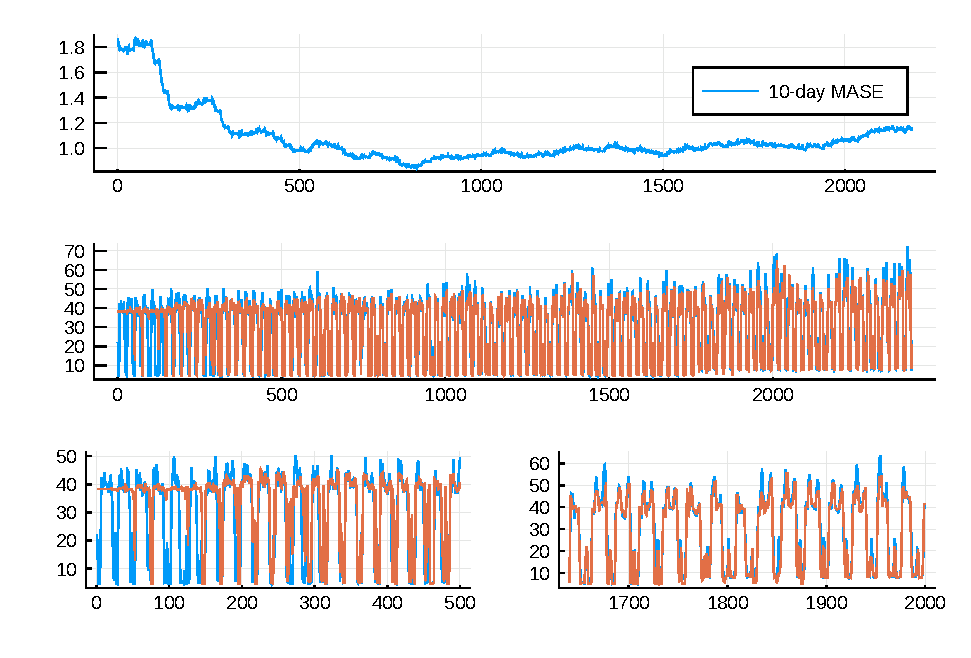
\includegraphics[width=1.05\textwidth,height=.6\textheight]{figures/tm1.eps}
		\caption[μελέτη πρόβλεψης χρονοσειράς με τη χρονική μνήμη]{%
			Μελέτη πρόβλεψης χρονοσειράς με τη χρονική μνήμη.
			Πάνω: εξέλιξη σφάλματος MASE σταθμισμένο σε διάστημα 10 ημερών.
			Μέση: {\color{blue}Χρονοσειρά} και {\color{red} πρόβλεψη}.
			Κάτω: εστίαση του παραπάνω στην αρχική εκμάθηση και στο σημείο αλλαγής της μέσης τιμής.
		}
		\label{fig:tm_tspredict}
	\end{figure}

	\begin{figure}[t]
		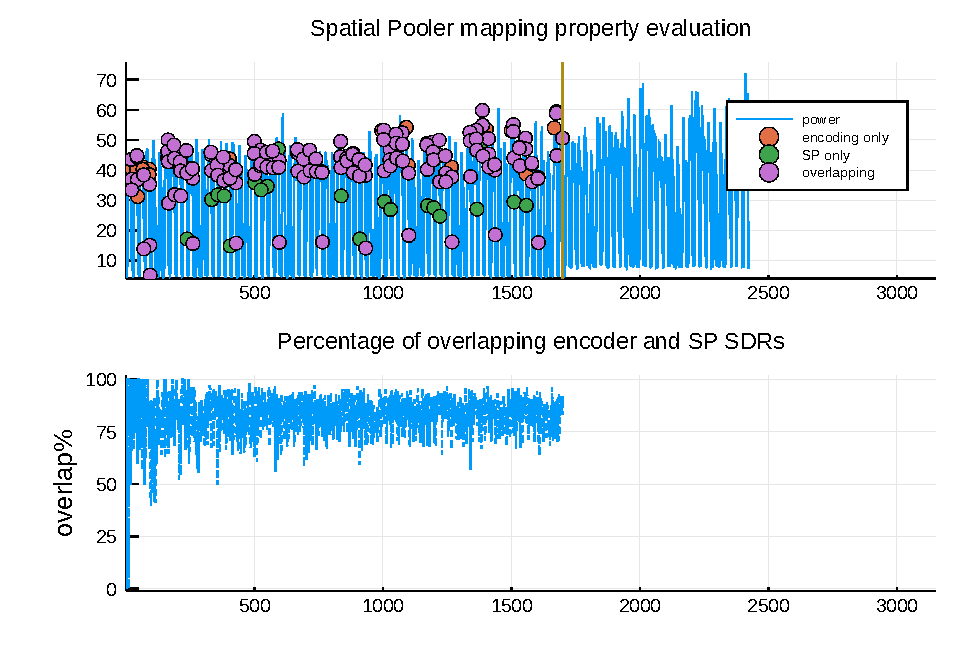
\includegraphics[width=1.1\textwidth]{figures/sp1.eps}
		\includegraphics[width=1.1\textwidth]{figures/sp2.eps}
		\caption[]{Μελέτη διατήρησης ομοιότητας του χώρου εισόδου από το χωρικό συγκεντρωτή
		-- αμέσως πριν και μετά την αλλαγή μέσης τιμής της χρονοσειράς}
	\end{figure}
	\begin{figure}[t]\ContinuedFloat
		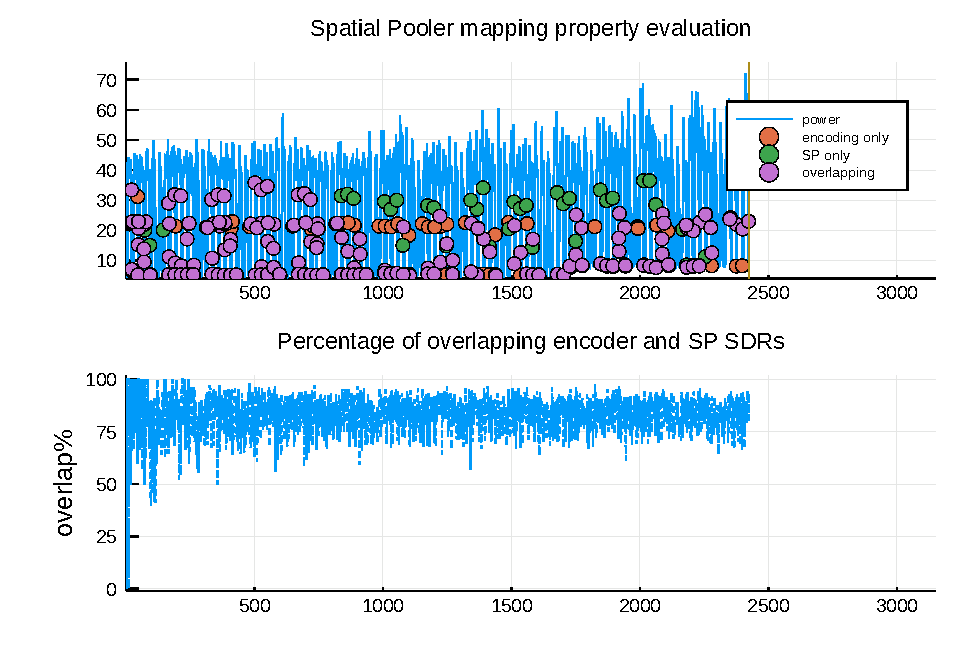
\includegraphics[width=1.1\textwidth]{figures/sp3.eps}

		\captionsetup{singlelinecheck=off}
		\caption[μελέτη διατήρησης ομοιότητας του χώρου εισόδου από το χωρικό συγκεντρωτή]{%
			Μελέτη διατήρησης ομοιότητας από το χώρο εισόδου στο χώρο εξόδου διαμέσου του χωρικού συγκεντρωτή. Αυτή είναι βασική αρχή λειτουργίας του χωρικού συγκεντρωτή
			και η απόδειξη της σχετικής της ισχύος χρησιμεύει τόσο ως τεκμήριο ορθότητας της υλοποίησης,
			όσο και του αλγορίθμου γενικότερα.
			Χρησιμοποιείται η χρονοσειρά που περιγράφεται στο \ref{conc:tspred-dataset}.

			Παρουσιάζονται 3 στιγμιότυπα: αμέσως πριν και αμέσως μετά την αλλαγή της μέσης τιμής της χρονοσειράς και στο τέλος.
			Για κάθε στιγμιότυπο υπάρχουν 2 γραφήματα.

			Στο πάνω φαίνεται η χρονοσειρά και επισημαίνονται τα πιο ταιριαστά ως τώρα SDR με την τρέχουσα στιγμή:
			{\color{red} είσοδοι που δεν ταιριάζουν πολύ με την τωρινή έξοδο},
			{\color{green} έξοδοι που δεν ταιριάζουν πολύ με την τωρινή είσοδο},
			{\color{magenta} είσοδοι και έξοδοι που ταιριάζουν με τις τωρινές}.

			Στο κάτω φαίνεται το ποσοστό των εισόδων/εξόδων που ταιριάζουν. Χρησιμεύει ως μέτρο επίδοσης του χωρικού συγκεντρωτή.

			Φαίνεται πως η αλλαγή της μέσης τιμής έχει αμελητέα επίδραση στην επίδοση του χωρικού συγκεντρωτή.
			Καθώς το πείραμα εξελίσσεται το μέτρο επίδοσης γίνεται πιο εύρωστο, καθώς προκύπτει από περισσότερα SDR.
			Αυτός είναι ο κύριος λόγος που μειώνεται η διακύμανση.
		}
		\label{fig:sp_maintain_similarity}
	\end{figure}


\section{Τι αξίζει να μελετηθεί περαιτέρω;} \label{conc:study-suggestions}

\subsubsection{Αισθητικοκινητική συμπερασματολογία και χρονική συγκέντρωση}

	Οι αλγόριθμοι που παρουσιάστηκαν εδώ αναπτύχθηκαν κυρίως μέχρι τις αρχές του 2017.
	Έκτοτε, η εταιρία Numenta που ηγείται της μελέτης έχει προτείνει πολλές νέες διαστάσεις στη θεωρία HTM.
	Βασική τέτοια είναι η αισθητικοκινητική συμπερασματολογία (sensorimotor inference).
	Βασιζόμενοι στην παρατήρηση ότι η είσοδος σε ένα ενσώματο σύστημα HTM μπορεί να αλλάζει για δύο διαφορετικούς λόγους,
	εξωγενή αλλαγή ή αλλαγή οπτικής γωνίας λόγω κίνησης του ιδίου του σώματος,
	προτείνουν ότι η διαδικασία της πρόβλεψης πρέπει να έχει πρόσβαση σε αντίγραφα των κινητικών εντολών και να τις λαμβάνει υπόψιν \parencite{hawkinsTheoryHowColumns2017}.
	Επίσης εισάγεται η έννοια της θέσης, τόσο του σώματος μέσα στον έξω κόσμο (πχ στο δωμάτιο), όσο και του αισθητήρα ως προς το αντικείμενο.
	Με αυτά τα στοιχεία συντίθεται η δυνατότητα μερικών φλοιικών στηλών που εργάζονται συντονισμένα να δημιουργήσουν μοντέλα φυσικών αντικειμένων και να τα διαχωρίσουν μεταξύ τους.

	Το μοντέλο του φυσικού αντικειμένου συσχετίζεται άμεσα με το μοντέλο μιας ακολουθίας στη χρονική μνήμη.
	Μία προέκταση της θεωρίας HTM που έχει κάποιο θεωρητικό υπόβαθρο αυτή τη στιγμή και χρήζει άμεσης μελέτης είναι
	ο συνδυασμός της χρονικής μνήμης με μία δεύτερη περιοχή που θα μοντελοποιεί ολόκληρες ακολυοθίες εισόδων
	και θα προδιαθέτει τη χρονική μνήμη με ανάδραση από τους κορυφαίους δενδρίτες.
	Ο μηχανισμός αυτός μπορεί να ονομαστεί και «χρονική συγκέντρωση» (temporal pooling).
	Στο παράδειγμα της παρακολούθησης μιας μελωδίας, αν η χρονική μνήμη μαθαίνει να αναπαριστά την τρέχουσα νότα ως προς τις προηγούμενες,
	ο χρονικός συγκεντρωτής μαθαίνει να αναπαριστά μουσικά θέματα.
	Η επιτυχής ενσωμάτωση ενός τέτοιου μηχανισμού αναμένεται να βελτιώσει σημαντικά την ικανότητα πρόβλεψης χρονοσειρών.

	Η χρονική μνήμη όπως παρουσιάστηκε, αν και δεν είναι ευαίσθητη στο θόρυβο του χώρου εισόδου χάρη στο χρονικό συγκεντρωτή,
	είναι πολύ ευαίσθητη στο \textbf{χρονικό θόρυβο}, όπως η ανταλλαγή της σειράς δύο συμβόλων εισόδου.
	Η προδιάθεση από το χρονικό συγκεντρωτή αναμένεται να προσδώσει ευρωστία σε τέτοιας μορφής θορύβου.

	Στο άρθρο \cite{hawkinsTheoryHowColumns2017} παρουσιάζεται μεν ένας μηχανισμός με τον οποίο η HTM μαθαίνει και αναγνωρίζει πολλά ξεχωριστά αντικείμενα,
	αλλά μονάχα με τη βοήθεια εξωγενούς σήμανσης για το πότε τα αντικείμενα αλλάζουν.
	Δεν περιγράφεται δηλαδή μηχανισμός \textbf{συνεχούς μάθησης}, με τον οποίο να μαθαίνονται και τα σύνορα μεταξύ των αντικειμένων.
	Σημαντικό ρόλο σε αυτήν την κατεύθυνση ενδέχεται να διαδραματίσει κάποιος μηχανισμός «έκπληξης», όπως είναι η έξαρση των μικροστηλών της χρονικής μνήμης
	για απροσδόκητες εισόδους.

\subsubsection{Ιεραρχική σύνθεση πολλών περιοχών}

	Αν και το όνομα της θεωρίας ξεκινά με τη λέξη «ιεραρχική», η ιεραρχία δε συμμετείχε σε όσα περιγράφηκαν ως τώρα.
	Η ιεραρχία αρχίζει να συντίθεται στην τρέχουσα θεωρία με ένα πρόσφατο άρθρο \cite{hawkinsFrameworkIntelligenceCortical2019}
	που προτείνει μηχανισμούς συνεργασίας πολλών φλοιικών στηλών.

	Σε πιο πρακτικό επίπεδο, η ιεραρχία φαίνεται να είναι το κλειδί για την πρόβλεψη και αναγνώριση ανωμαλιών σε πολύπλοκα συστήματα
	που εκφράζουν τη συνολική τους κατάσταση με πολλές ταυτόχρονες χρονοσειρές (\textbf{multivariate timeseries prediction}).
	Με μία μόνο περιοχή δεν υπάρχει αποτελεσματικός τρόπος για τη σύνθεση πολλών χρονοσειρών σε ένα χώρο εισόδου.

\subsubsection{Διάφορες ιδέες}

	Οι παραπάνω είναι ίσως οι πιο σημαντικές κατευθύνσεις για περαιτέρω έρευνα, όμως αναγνωρίζονται και πολλά πιο εντοπισμένα ερωτήματα
	ως προς τη συμπεριφορά των αλγορίθμων που περιγράφηκαν.
	\begin{itemize}
		\item Είναι ευσταθείς οι μηχανισμοί εκμάθησης; Πώς επηρεάζονται από τον κβραντισμό των συναπτικών μονιμοτήτων;
		\item Αν δούμε το δίκτυο της χρονικής μνήμης ως γράφο με τοπικούς κανόνες προσαρμογής, είναι ενδιαφέρον να μελετηθεί υπό το πρίσμα του άρθρου \cite{kipouridisConvergenceNetworkSystems2019}
		\item Οι συνάψεις αυτή τη στιγμή είναι δισταθείς (συνδεδεμένες/αποσυνδεδεμένες), αλλά ο μόνος βιολογικός περιορισμός είναι ότι δεν μπορούν να έχουν μεγάλη ακρίβεια.
		Ας μελετηθούν λοιπόν συνάψεις με περισσότερες καταστάσεις, με συναπτικά βάρη 2-3 bit.
	\end{itemize}

	Τέλος, όσον αφορά την παρούσα υλοποίηση, οι ιδιότητες των αλγορίθμων επικυρώθηκαν μόνο αδρομερώς με δύο συνολικούς ελέγχους.
	Η επίσημη υλοποίηση της Numenta έχει μελετηθεί με πολύ περισσότερους ελέγχους, που παρουσιάζονται στα άρθρα τους
	\parencite{cuiHTMSpatialPooler2017,cuiContinuousOnlineSequence2016}.
	Είναι σημαντικό να αναπαραχθούν αυτοί οι έλεγχοι, ώστε να τεκμηριωθούν και οι υπόλοιπες ιδιότητες του χωρικού συγκεντρωτή και της χρονικής μνήμης.


\section{Συμπέρασμα}

	Στην εργασία αυτή παρουσιάστηκε η θεωρία HTM, μαζί με το βιολογικό υπόβαθρο που προσπαθεί να ερμηνεύσει,
	και μια υλοποίηση των κεντρικών της αλγορίθμων σε νέα γλώσσα μαθηματικού προγραμματισμού, τη Julia.

	Οι αλγόριθμοι είναι περίπλοκοι και σχετικά πολύπλοκοι, όχι ως προς την υπολογιστική τους πολυπλοκότητα,
	αλλά ως προς τη δυσκολία στην περιγραφή των πολλών εννοιών που περιλαμβάνουν.
	Η υλοποίηση του χωρικού συγκεντρωτή σε 120 γραμμές κώδικα και της χρονικής μνήμης σε 222,
	σε αντιδιαστολή με την πρότυπη υλοποίηση των αλγορίθμων σε 700 και 750 γραμμές αντίστοιχα,
	θεωρείται ότι μπορεί να αποτελέσει μια αποτελεσματική περίληψη των αλγορίθμων και ταυτόχρονα σαφή τους διατύπωση.
	Η επιτυχία του κεντρικού αυτού στόχου της εργασίας, όμως, θα μπορέσει να αξιολογηθεί μόνο στο μέλλον, με το κατά πόσον πράγματι θα αποτελέσει βάση για περαιτέρω μελέτη.

	Η υλοποίηση απαιτούσε τη βαθιά κατανόηση της Julia.
	Χρησιμοποιήθηκαν και παρουσιάστηκαν προχωρημένες δυνατότητες της γλώσσας όπως μοτίβα σχεδιασμού με παραμετρικές μεθόδους και πολλαπλή αποστολή,
	χαμηλού επιπέδου χειρισμοί με αραιούς πίνακες, μακροεντολές, μετρήσεις απόδοσης (benchmarking) και άλλα.
	Οδήγησε επίσης στη συνεισφορά στην πηγή της επίλυσης μερικών προβλημάτων, στο πλαίσιο της ανάπτυξης ενός παγκόσμιου εύρους ανοιχτού λογισμικού.

	Οι αλγόριθμοι δοκιμάστηκαν με βασικούς ελέγχους και η λειτουργικότητά τους επιδείχτηκε.
	Παρατηρήθηκε βέβαια ότι, στην παρούσα μορφή, δεν είναι ιδιαίτερα αποτελεσματικοί στο πρόβλημα της πρόβλεψης,
	και ότι χρειάζονται περισσότερη μελέτη και πειραματισμό με ήδη προταθείσες θεωρητικές βελτιώσεις.

	Εν τέλει, αναφέρθηκαν πιθανές προεκτάσεις για περαιτέρω μελέτη, καταδεικνύοντας και πώς ενδέχεται να βελτιωθεί η απόδοση των αλγορίθμων
	και πώς αυτή η εργασία μπορεί να φανεί χρήσιμη.


\printbibliography

%\begin{appendices}
%\chapter{Τμήματα κώδικα}
%\input{chapters/app_codesnip.tex}
%\end{appendices}

\end{document}
